%%%%%%%%%%%%%%%%%%%%%%%%%%%%%%%%%%%%%%%%
%% Compile: PDFLaTeX BibTeX PDFLaTeX(x2)
%%%%%%%%%%%%%%%%%%%%%%%%%%%%%%%%%%%%%%%%

\documentclass[a4paper,11pt, bibtotoc]{beamer}
%\documentclass[10pt,a4paper]{beamer}
%\documentclass[10pt,handout]{beamer}

%%%%%%%%%%%%%%%%%%%%%%%%
%%     PACKAGES       %%
%%%%%%%%%%%%%%%%%%%%%%%%

%%%%%%%%%%%%%%%%%%%%%%%%
%%     PACKAGES       %%
%%%%%%%%%%%%%%%%%%%%%%%%



%\usepackage[utf8]{inputenc}
%\usepackage[vietnamese, english,ngerman]{babel}   % seems incompatible with german.sty
%\usepackage[T3,T1]{fontenc} breaks xelatex
\usepackage{lmodern}

\usepackage{amsmath}
\usepackage{amsfonts}
\usepackage{amssymb}
%% MnSymbol: Mathematische Klammern und Symbole (Inkompatibel mit ams-Packages!)
%% Bedeutungs- und Graphemklammern: $\lsem$ Tisch $\rsem$ $\langle TEXT \rangle$ $\llangle$ TEXT $\rrangle$ 
\usepackage{MnSymbol}
%% ulem: Strike out
\usepackage[normalem]{ulem}  

%% Special Spaces (s. Commands)
\usepackage{xspace}				
\usepackage{setspace}
%	\onehalfspacing

%% mdwlist: Special lists
\usepackage{mdwlist}	

\usepackage[noenc,safe]{tipa}

% maybe define \textipa to use \originalTeX to avoid problems with `"'.
%
%	\ex \textipa{\originalTeX [pa.pa."g\t{aI}]}

%

\usepackage{etex}		%For Forest bug

%
%\usepackage{jambox}
%


%\usepackage{forest-v105}
%\usepackage{modified-langsci-forest-setup}

\usepackage{xeCJK}
\setCJKmainfont{SimSun}


%\usepackage{natbib}
%\setcitestyle{notesep={:~}}




% for toggles
\usepackage{etex}



% Fraktur!
\usepackage{yfonts}

\usepackage{url}

% für UDOP
\usepackage{adjustbox}


%% huberlin: Style sheet
%\usepackage{huberlin}
\usepackage{hu-beamer-includes-pdflatex}
\huberlinlogon{0.86cm}


%% Last Packages
%\usepackage{hyperref}	%URLs
%\usepackage{gb4e}		%Linguistic examples

% sorry this was incompatible with gb4e and had to go.
%\usepackage{linguex-cgloss}	%Linguistic examples (patched version that works with jambox

\usepackage{multirow}  %Mehrere Zeilen in einer Tabelle
%\usepackage{array}
\usepackage{marginnote}	%Notizen




%%%%%%%%%%%%%%%%%%%%%%%%%%%%%%%%%%%%%%%%%%%%%%%%%%%%
%%%             Preamble's End                   %%%
%%%%%%%%%%%%%%%%%%%%%%%%%%%%%%%%%%%%%%%%%%%%%%%%%%%% 

\begin{document}

%%%%%%%%%%%%%%%%%%%%%%%%%%%%%%%%%%%%%%%%%%%%%%%%%%%%
%%%          Commands                            %%%
%%%%%%%%%%%%%%%%%%%%%%%%%%%%%%%%%%%%%%%%%%%%%%%%%%%%

%%%%%%%%%%%%%%%%%%%%%%%%%%%%%%%%
% German quotation marks:
\newcommand{\gqq}[1]{\glqq{}#1\grqq{}}		%double
\newcommand{\gq}[1]{\glq{}#1\grq{}}			%simple


%%%%%%%%%%%%%%%%%%%%%%%%%%%%%%%%
% Abbreviations in German
% package needed: xspace
% Short space in German abbreviations: \,	
\newcommand{\idR}{\mbox{i.\,d.\,R.}\xspace}
\newcommand{\su}{\mbox{s.\,u.}\xspace}
%\newcommand{\ua}{\mbox{u.\,a.}\xspace}       % in abbrev
%\newcommand{\zB}{\mbox{z.\,B.}\xspace}       % in abbrev
%\newcommand{\s}{s.~}
%not possibel: \dh --> d.\,h.


%%%%%%%%%%%%%%%%%%%%%%%%%%%%%%%%
%Abbreviations in English
\newcommand{\ao}{a.o.\ }	% among others
\newcommand{\cf}[1]{(cf.~#1)}	% confer = compare
\renewcommand{\ia}{i.a.}	% inter alia = among others
\newcommand{\ie}{i.e.~}	% id est = that is
\newcommand{\fe}{e.g.~}	% exempli gratia = for example
%not possible: \eg --> e.g.~
\newcommand{\vs}{vs.\ }	% versus
\newcommand{\wrt}{w.r.t.\ }	% with respect to


%%%%%%%%%%%%%%%%%%%%%%%%%%%%%%%%
% Dash:
\newcommand{\gs}[1]{--\,#1\,--}


%%%%%%%%%%%%%%%%%%%%%%%%%%%%%%%%
% Rightarrow with and without space
\def\ra{\ensuremath\rightarrow}			%without space
\def\ras{\ensuremath\rightarrow\ }		%with space


%%%%%%%%%%%%%%%%%%%%%%%%%%%%%%%%
%% X-bar notation

%% Notation with primes (not emphasized): \xbar{X}
\newcommand{\MyPxbar}[1]{#1$^{\prime}$}
\newcommand{\xxbar}[1]{#1$^{\prime\prime}$}
\newcommand{\xxxbar}[1]{#1$^{\prime\prime\prime}$}

%% Notation with primes (emphasized): \exbar{X}
\newcommand{\exbar}[1]{\emph{#1}$^{\prime}$}
\newcommand{\exxbar}[1]{\emph{#1}$^{\prime\prime}$}
\newcommand{\exxxbar}[1]{\emph{#1}$^{\prime\prime\prime}$}

% Notation with zero and max (not emphasized): \xbar{X}
\newcommand{\zerobar}[1]{#1$^{0}$}
\newcommand{\maxbar}[1]{#1$^{\textsc{max}}$}

% Notation with zero and max (emphasized): \xbar{X}
\newcommand{\ezerobar}[1]{\emph{#1}$^{0}$}
\newcommand{\emaxbar}[1]{\emph{#1}$^{\textsc{max}}$}

%% Notation with bars (already implemented in gb4e):
% \obar{X}, \ibar{X}, \iibar{X}, \mbar{X} %Problems with \mbar!
%
%% Without gb4e:
\newcommand{\overbar}[1]{\mkern 1.5mu\overline{\mkern-1.5mu#1\mkern-1.5mu}\mkern 1.5mu}
%
%% OR:
\newcommand{\MyPibar}[1]{$\overline{\textrm{#1}}$}
\newcommand{\MyPiibar}[1]{$\overline{\overline{\textrm{#1}}}$}
%% (emphasized):
\newcommand{\eibar}[1]{$\overline{#1}$}
\newcommand{\eiibar}[1]{\overline{$\overline{#1}}$}

%%%%%%%%%%%%%%%%%%%%%%%%%%%%%%%%
%% Subscript & Superscript: no italics
\newcommand{\MyPdown}[1]{$_{\textrm{#1}}$}
\newcommand{\MyPup}[1]{$^{\textrm{#1}}$}


%%%%%%%%%%%%%%%%%%%%%%%%%%%%%%%%
% Objekt language marking:
%\newcommand{\obj}[1]{\glqq{}#1\grqq{}}	%German double quotes
%\newcommand{\obj}[1]{``#1''}			%English double quotes
\newcommand{\MyPobj}[1]{\emph{#1}}		%Emphasising


%%%%%%%%%%%%%%%%%%%%%%%%%%%%%%%%
%% Semantic types (<e,t>), features, variables and graphemes in angled brackets 

%%% types and variables, in math mode: angled brackets + italics + no space
%\newcommand{\type}[1]{$<#1>$}

%%% OR more correctly: 
%%% types and variables, in math mode: chevrons! + italics + no space
\newcommand{\MyPtype}[1]{$\langle #1 \rangle$}

%%% features and graphemes, in math mode: chevrons! + italics + no space
\newcommand{\abe}[1]{$\langle #1 \rangle$}


%%% features and graphemes, in math mode: chevrons! + no italics + space
\newcommand{\ab}[1]{$\langle$#1$\rangle$}  %%same as \abu  
\newcommand{\abu}[1]{$\langle$#1$\rangle$} %%Umlaute

%%% Notizen
\renewcommand{\marginfont}{\singlespacing}
\renewcommand{\marginfont}{\footnotesize}
\renewcommand{\marginfont}{\color{black}}

\newcommand{\myp}[1]{%
	\marginnote{%
		\begin{spacing}{1}
			\vspace{-\baselineskip}%
			\color{red}\footnotesize#1
		\end{spacing}
	}
}
%%%%%%%%%%%%%%%%%%%%%%%%%%%%%%%%
%% Outputbox
\newcommand{\outputbox}[1]{\noindent\fbox{\parbox[t][][t]{0.98\linewidth}{#1}}\vspace{0.5em}}

%%%%%%%%%%%%%%%%%%%%%%%%%%%%%%%%
%% (Syntactic) Trees
% package needed: forest
%
%% Setting for simple trees
\forestset{
	MyP edges/.style={for tree={parent anchor=south, child anchor=north}}
}

%% this is taken from langsci-setup file
%% Setting for complex trees
%% \forestset{
%% 	sn edges/.style={for tree={parent anchor=south, child anchor=north,align=center}}, 
%% background tree/.style={for tree={text opacity=0.2,draw opacity=0.2,edge={draw opacity=0.2}}}
%% }

\newcommand\HideWd[1]{%
	\makebox[0pt]{#1}%
}


%%%%%%%%%%%%%%%%%%%%%%%%%%%%%%%%%%%%%%%%%%%%%%%%%%%%
%%%          Useful commands                     %%%
%%%%%%%%%%%%%%%%%%%%%%%%%%%%%%%%%%%%%%%%%%%%%%%%%%%%

%%%%%%%%%%%%%%%%%%%%%
%% FOR ITEMS:
%\begin{itemize}
%  \item<2-> from point 2
%  \item<3-> from point 3 
%  \item<4-> from point 4 
%\end{itemize}
%
% or: \onslide<2->
% or: \pause

%%%%%%%%%%%%%%%%%%%%%
%% VERTICAL SPACE:
% \vspace{.5cm}
% \vfill

%%%%%%%%%%%%%%%%%%%%%
% RED MARKING OF TEXT:
%\alert{bis spätestens Mittwoch, 18 Uhr}

%%%%%%%%%%%%%%%%%%%%%
%% RESCALE BIG TABLES:
%\scalebox{0.8}{
%For Big Tables
%}

%%%%%%%%%%%%%%%%%%%%%
%% BLOCKS:
%\begin{alertblock}{Title}
%Text
%\end{alertblock}
%
%\begin{block}{Title}
%Text
%\end{block}
%
%\begin{exampleblock}{Title}
%Text
%\end{exampleblock}


\newtoggle{uebung}
\newtoggle{loesung}
\newtoggle{toc}

% The toc is not needed on Handouts. Safe trees.
\mode<handout>{
\togglefalse{toc}
}

\newtoggle{hpsgvorlesung}\togglefalse{hpsgvorlesung}
\newtoggle{syntaxvorlesungen}\togglefalse{syntaxvorlesungen}

%\includecomment{psgbegriffe}
%\excludecomment{konstituentenprobleme}
%\includecomment{konstituentenprobleme-hinweis}

\newtoggle{konstituentenprobleme}\togglefalse{konstituentenprobleme}
\newtoggle{konstituentenprobleme-hinweis}\toggletrue{konstituentenprobleme-hinweis}

%\includecomment{einfsprachwiss-include}
%\excludecomment{einfsprachwiss-exclude}
\newtoggle{einfsprachwiss-include}\toggletrue{einfsprachwiss-include}
\newtoggle{einfsprachwiss-exclude}\togglefalse{einfsprachwiss-exclude}

\newtoggle{psgbegriffe}\toggletrue{psgbegriffe}

\newtoggle{gb-intro}\togglefalse{gb-intro}



%%%%%%%%%%%%%%%%%%%%%%%%%%%%%%%%%%%%%%%%%%%%%%%%%%%%
%%%             Metadata                         %%%
%%%%%%%%%%%%%%%%%%%%%%%%%%%%%%%%%%%%%%%%%%%%%%%%%%%%      

\title{\textbf{Grundkurs Linguistik}}

\subtitle{Phonologie II: Silbe}

\author[aMyP]{
	{\small Antonio Machicao y Priemer}
%	\\
%	{\footnotesize \url{http://www.linguistik.hu-berlin.de/staff/amyp}\\
%	\href{mailto:mapriema@hu-berlin.de}{mapriema@hu-berlin.de}}
}

\institute{Institut für deutsche Sprache und Linguistik}

%%%%%%%%%%%%%%%%%%%%%%%%%      
\date{ }
%\publishers{\textbf{6. linguistischer Methodenworkshop \\ Humboldt-Universität zu Berlin}}

%\hyphenation{nobreak}


%%%%%%%%%%%%%%%%%%%%%%%%%%%%%%%%%%%%%%%%%%%%%%%%%%%%
%%%             Preamble's End                   %%%
%%%%%%%%%%%%%%%%%%%%%%%%%%%%%%%%%%%%%%%%%%%%%%%%%%%%      


%%%%%%%%%%%%%%%%%%%%%%%%%      
\begin{frame}
  \HUtitle
\end{frame}

\frame{
\begin{multicols}{2}
	\frametitle{Inhaltsverzeichnis}\tableofcontents
	%[pausesections]
\end{multicols}
}

%%%%%%%%%%%%%%%%%%%%%%%%%%%%%%%%%%%
%%%%%%%%%%%%%%%%%%%%%%%%%%%%%%%%%%
\section{Kontakt}
%\frame{
%\begin{multicols}{2}
%\frametitle{~}
%	\tableofcontents[currentsection]
%\end{multicols}
%}
%%%%%%%%%%%%%%%%%%%%%%%%%%%%%%%%%%

\begin{frame}
\frametitle{Kontakt}


\scalebox{0.95}{

\begin{tabular}{ll}
\textbf{Dozent:} & Antonio Machicao y Priemer \\ 
			     & \textipa{[ma.\t{tS}i."ka.o.\textprimstress Pi."p\textscr i:.m5]}\\
\textbf{E-Mail:} & \href{mailto:mapriema@hu-berlin.de}{mapriema@hu-berlin.de} \\ 
\textbf{Webseite:} & \url{http://www.linguistik.hu-berlin.de/staff/amyp} \\ 
\textbf{Büro:} & Dorotheenstraße 24, Raum: 3.305 \\ 
\textbf{Telefonnummer:} & +49(30)-2093-9702 \\
\textbf{Sprechstunde:} & Mittwochs 10--12 (Anmeldung per E-Mail erforderlich!) \\ 
 & \\
\textbf{Sekretariat:} & Anina Klein \\	
\textbf{E-Mail:} & \href{mailto:Anina.Klein@cms.hu-berlin.de}{Anina.Klein@cms.hu-berlin.de} \\
\textbf{Büro:} & Dorotheenstraße 24, Raum: 3.306 \\
\textbf{Telefonnummer:} & +49(30)-2093-9639 \\
\end{tabular} 

}
\end{frame}



%%%%%%%%%%%%%%%%%%%%%%%%%%%%%%%%%%
%%%%%%%%%%%%%%%%%%%%%%%%%%%%%%%%%%
\section{Einführung}
%\frame{
%\begin{multicols}{2}
%\frametitle{~}
%	\tableofcontents[currentsection]
%\end{multicols}
%}
%%%%%%%%%%%%%%%%%%%%%%%%%%%%%%%%%%%
%% LITERATUR
\nocite{Altmann&Co07a} \nocite{Hall00a} \nocite{Pompino95a} \nocite{Ramers08a} \nocite{Repp&Co12a} \nocite{WieseR96a} \nocite{WieseR11a}
%%%%%%%%%%%%%%%%%%%%%%%%%%%%%%%%%%%
%%%%%%%%%%%%%%%%%%%%%%%%%%%%%%%%%%%

\begin{frame}
\frametitle{Einführung}


\begin{itemize}
	\item Graphematische Notation in spitzen Klammern: 
	
	\ex. \ab{nordwind}, \ab{Nordwind}

	\item[]	
	\item Phonetische Notation in eckigen Klammern:
	
	\ex. \textipa{[nO5t.vInt]}
	
	\item[]
	\item Phonologische Notation in Schrägstrichen:
	
	\ex. \textipa{/nO\textscr d.vInd/}
	
\end{itemize}

\end{frame}



%%%%%%%%%%%%%%%%%%%%%%%%%%%%%%%%%%%
\begin{frame}
\frametitle{Einführung}


Warum nimmt man Silben an?

\begin{itemize}
	\item Die Auslautverhärtung mit Bezug auf das Wort (vorläufig):
	
	\ex. [$-$son] $\rightarrow$ [$-$sth] /\_\_ \#
	
	\item Transkribieren Sie: \emph{(sie) siegte}
\pause	
	\ex. \textipa{[zi:k . t@]} (\gqq{.} steht für Silbengrenze)

\pause
	\ex. 
	\a. \textipa{[St\textscr e:p.za:m]} \vs. \textipa{[St\textscr e:.b5]}
	\b. \textipa{[bYnt.nIs]} \vs \textipa{[bUn.d@s]}
	\b. \textipa{[bi:k.za:m]} \vs \textipa{[bi:.g@n]}
	\b. \textipa{[le:s.b5]} \vs \textipa{[le:.z@n]}

	\item Auslautverhärtung mit Bezug auf die \textbf{Silbe}:
	\ex. [$-$son] $\rightarrow$ [$-$sth] /\_\_ $]_{\sigma}$
		
\end{itemize}


\end{frame}



%%%%%%%%%%%%%%%%%%%%%%%%%%%%%%%%%%%

\begin{frame}
\frametitle{Einführung}

Warum nimmt man Silben an?

Silbe als \textbf{Domäne} \dots

\begin{itemize}	
	\item \dots\ verschiedener \textbf{phonologischer Prozesse} (\zB Auslautverhärtung, Knacklauteinsetzung, Aspiration, \dots )
	
	\item[] 
	
	\item \dots\ von Regularitäten bzgl. der \textbf{Abfolge} von Lauten
	
	\item[]
	
	\item \dots\ der \textbf{Wortbetonung}, d.\,h. wichtige so genannte prosodische Einheiten (Prosodie = Bezug auf Einheiten über dem Segment)
\end{itemize}

\end{frame}



%%%%%%%%%%%%%%%%%%%%%%%%%%%%%%%%%%%

\begin{frame}
\frametitle{Einführung}


\begin{itemize}
	\item Prosodische Konstituenten:
	\begin{multicols}{2}
	\begin{itemize}
		\item UP = Äußerungsphrase
		\item IP = Intonationsphrase
		\item $\phi$ = phonol. Phrase
\columnbreak
		\item $\omega$ = phonol. Wort
		\item F = phonol. Fuß
		\item \alert{$\sigma$ = Silbe}
	\end{itemize}
	\end{multicols}
\end{itemize}

\begin{figure}[b]
	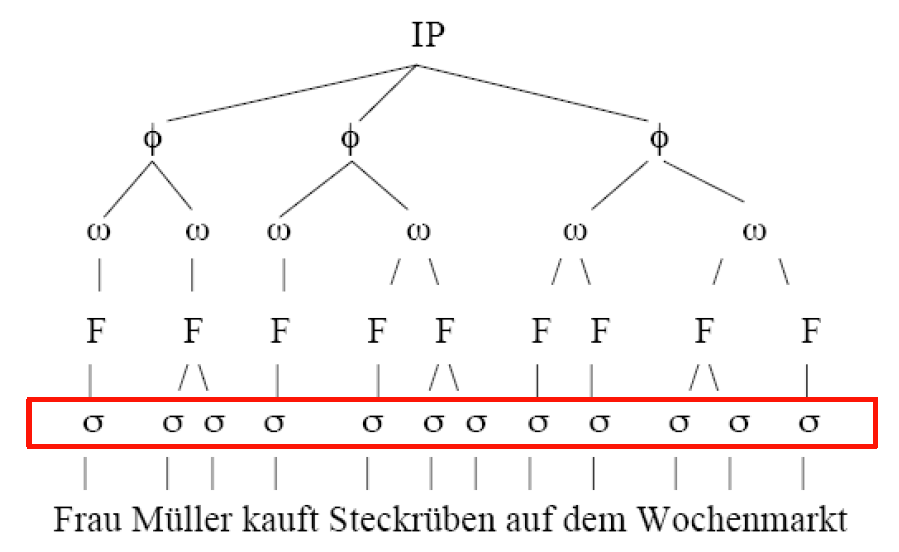
\includegraphics[scale=0.32]{../material/03bHierarchieIntonationsphrase}
	\caption{Hierarchie in der Intonationsphrase (Darstellung von C. Féry)}
	\label{Zeichen1}
\end{figure}

\end{frame}



%%%%%%%%%%%%%%%%%%%%%%%%%%%%%%%%%%%

\begin{frame}
\frametitle{Einführung}


\begin{itemize}
	\item Prosodische Konstituenten:
	\begin{multicols}{2}
	\begin{itemize}
		\item UP = Äußerungsphrase
		\item IP = Intonationsphrase
		\item $\varphi$ = phonol. Phrase
\columnbreak
		\item $\omega$ = phonol. Wort
		\item F = phonol. Fuß
		\item \alert{$\sigma$ = Silbe}
	\end{itemize}
	\end{multicols}
\end{itemize}

\begin{figure}[b]
	\centering
	
	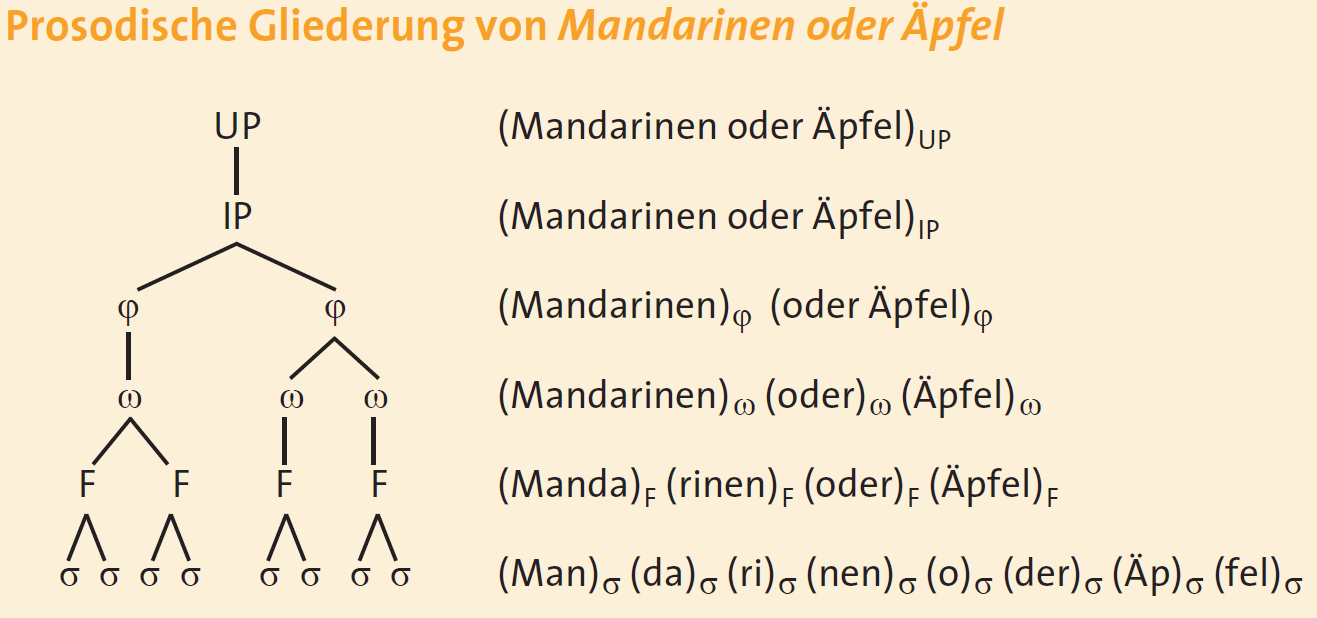
\includegraphics[scale=0.28]{../material/03bHierarchieUP}
	\caption{Hierarchie in der Äußerungsphrase \citep[8]{Fuhrhop&Co13a}}
	%\label{Zeichen1}
\end{figure}


\end{frame}



%%%%%%%%%%%%%%%%%%%%%%%%%%%%%%%%%%
%%%%%%%%%%%%%%%%%%%%%%%%%%%%%%%%%%
\section{Silbenbestimmung}
%\frame{
%\frametitle{~}
%\begin{multicols}{2}
%	\tableofcontents[currentsection]
%\end{multicols}	
%}
%%%%%%%%%%%%%%%%%%%%%%%%%%%%%%%%%%

\begin{frame}
\frametitle{Silbenbestimmung}

\begin{itemize}
	\item Wie viele Silben hat das folgende Wort?
	
	\ex. Silbenbestimmung

\pause	
	\item Woher wissen Sie das?
	
	\begin{itemize}
		\item Staffeldt (2010: 133):\\
		\gqq{Jeder kompetente Sprachteilhaber verfügt über die \textbf{Fähigkeit}, Silben identifizieren zu können.}
		
		\item \citet[600]{Bussmann02a}:\\
		\gqq{Silbe: Phonetisch- phonologische \textbf{Grundeinheit} des Wortes bzw. der Rede, die zwar \textbf{intuitiv} nachweisbar ist, wissenschaftlich aber \textbf{nicht einheitlich definiert} wird.}
		
	\end{itemize}

	\item Silben können \textbf{betont} werden (tragen Akzent)
	
	\item Silbenspiele
	
	\item Intuitiv erkennbare Einheit

\end{itemize}

\end{frame}



%%%%%%%%%%%%%%%%%%%%%%%%%%%%%%%%%%
%%%%%%%%%%%%%%%%%%%%%%%%%%%%%%%%%%
\section{Silbenstruktur}
%\frame{
%\frametitle{~}
%\begin{multicols}{2}
%	\tableofcontents[currentsection]
%\end{multicols}	
%
%}
%%%%%%%%%%%%%%%%%%%%%%%%%%%%%%%%%%
\begin{frame}
\frametitle{Silbenstruktur}

\begin{itemize}
	\item Welche Silben (des Deutschen) sind mit den folgenden Segmenten bildbar?
	
	\ex. \textipa{[p]}, \textipa{[a]}, \textipa{[l]}, \textipa{[t]}
\pause	
	\a. Bildbar:\\
	\textipa{[palt]}, \textipa{[alpt]}, \textipa{[lapt]}, \textipa{[talp]}, \textipa{[plat]}
	\b. Nicht bildbar:\\
	*\textipa{[ltap]}, \dots\

\pause
	\item Warum?
\end{itemize}

\end{frame}



%%%%%%%%%%%%%%%%%%%%%%%%%%%%%%%%%%%
%\begin{frame}
%\frametitle{Silbenstruktur}
%
%Die Silbe ist \textbf{intern strukturiert} und besteht aus den folgenden Teilen:
%
%\begin{minipage}{.60\textwidth}
%
%\begin{itemize}
%	\item[]
%	\item Silbenanlaut / Silbenanfangsrand / \alert{Onset},
%	\begin{itemize}
%		\item 0 bis $n$ Konsonanten, wobei in fast allen Sprachen $n < 5$
%	\end{itemize}
%	
%	\item[]
%	\item Silbengipfel / Silbenkern / \alert{Nukleus},
%	\begin{itemize}
%		\item Vokale
%		\item manchmal (vokalische) Nasale oder Liquide
%	\end{itemize}
%	
%	\item[]
%	\item Silbenauslaut / Silbenendrand / \alert{Koda}
%	\begin{itemize}
%		\item 0 bis $n$ Konsonanten, wobei in fast allen Sprachen $n < 5$
%	\end{itemize}
%
%	\item[]
%	\item Nukleus und Koda bilden den \alert{Reim}
%	
%\end{itemize}
%
%
%\end{minipage}
%\begin{minipage}{.39\textwidth}
%
%%%%%%%%%%%%%%
%%% Forestset Syllables

\newbox\foreststrutbox
\setbox\foreststrutbox=\hbox to 0pt{\phantom{\forestOve{standard node}{content}}}
\def\foreststrut{\copy\foreststrutbox}
\forestset{
GP1/.style 2 args={
for n={1}{baseline},
s sep=0pt, l sep=0pt,
for descendants={
l sep=0pt, l={#1},
anchor=base,calign=first,child anchor=north,
inner xsep=1pt,inner ysep=2pt,outer sep=0pt,s sep=0pt,
},
delay={
if content={}{phantom}{for children={no edge}},
for tree={
if content={O}{tier=OR}{},
if content={R}{tier=OR}{},
if content={N}{tier=N}{},
if content={x}{
tier=x,content={$\times$},outer xsep={#2},
for tree={calign=center},
for descendants={content format={\foreststrut\forestoption{content}}},
before drawing tree={outer xsep=0pt,delay={typeset node}},
s sep=4pt
}{},
},
},
before drawing tree={where content={}{parent anchor=center,child anchor=center}{}},
},
GP1/.default={5ex}{8.0pt},
associate/.style={%
tikz+={\draw(!)--(!#1);}},
spread/.style={
before drawing tree={tikz+={\draw[dotted](!)--(!#1);}}},
govern/.style={
before drawing tree={tikz+={\draw[->](!)--(!#1);}}},
p-govern/.style={
before drawing tree={tikz+={\draw[->](.north) to[out=150,in=30] (!#1.north);}}},
no p-govern/.style={
before drawing tree={tikz+={\draw[->,loosely dashed](.north) to[out=150,in=30] (!#1.north);}}},
encircle/.style={before drawing tree={circle,draw,inner sep=0pt}},
fen/.style={pin={[font=\footnotesize,inner sep=1pt,pin edge=<-]10:\textsc{Fen}}},
el/.style={content=\textsc{\textbf{##1}}},
head/.style={content=\textsc{\textbf{\underline{##1}}}},
llap/.style={
tikz+={%
\edef\forest@temp{\noexpand\node[\option{node options},
anchor=base east,at=(.base east)]}%
\forest@temp{#1\phantom{\option{environment}}};
}
},
rlap/.style={
tikz+={%
\edef\forest@temp{\noexpand\node[\option{node options},
anchor=base west,at=(.base west)]}%
\forest@temp{\phantom{\option{environment}}#1};
}
},
}
%%%%%%%%%%%%%

%\begin{figure}
%\centering
%\begin{forest} sn edges, GP1 [
%  [$\sigma$
%    [O	[ [C$^{n}$]]
%    ]
%    [R	[N
%    		[V$^{n}$]
%    	]
%    	[K
%    		[C$^{n}$]
%    	]
%    ]
%  ]
%]
%\end{forest}
%\caption{Silbenstruktur}
%\end{figure}
%
%\end{minipage}
%
%\end{frame}



%%%%%%%%%%%%%%%%%%%%%%%%%%%%%%%%%%

\begin{frame}
\frametitle{Silbenstruktur}

Die Silbe ist \textbf{intern strukturiert} und besteht aus den folgenden Teilen:

\begin{minipage}{.59\textwidth}

\begin{itemize}
	\item[]
	\item \alert{Onset}
	
	\item \alert{Reim}
	
	\item \alert{Nukleus}
	
	\item \alert{Koda}
	\item[] 
	\item C $:=$ Konsonantisch, d.\,h. nicht-silbisch ($\neq$Konsonant)
	\item V $:=$ Vokalisch, d.\,h. silbisch ($\neq$Vokal)
	
\end{itemize}


\end{minipage}
\begin{minipage}{.40\textwidth}

%%%%%%%%%%%%%
%%% Forestset Syllables

\newbox\foreststrutbox
\setbox\foreststrutbox=\hbox to 0pt{\phantom{\forestOve{standard node}{content}}}
\def\foreststrut{\copy\foreststrutbox}
\forestset{
GP1/.style 2 args={
for n={1}{baseline},
s sep=0pt, l sep=0pt,
for descendants={
l sep=0pt, l={#1},
anchor=base,calign=first,child anchor=north,
inner xsep=1pt,inner ysep=2pt,outer sep=0pt,s sep=0pt,
},
delay={
if content={}{phantom}{for children={no edge}},
for tree={
if content={O}{tier=OR}{},
if content={R}{tier=OR}{},
if content={N}{tier=N}{},
if content={x}{
tier=x,content={$\times$},outer xsep={#2},
for tree={calign=center},
for descendants={content format={\foreststrut\forestoption{content}}},
before drawing tree={outer xsep=0pt,delay={typeset node}},
s sep=4pt
}{},
},
},
before drawing tree={where content={}{parent anchor=center,child anchor=center}{}},
},
GP1/.default={5ex}{8.0pt},
associate/.style={%
tikz+={\draw(!)--(!#1);}},
spread/.style={
before drawing tree={tikz+={\draw[dotted](!)--(!#1);}}},
govern/.style={
before drawing tree={tikz+={\draw[->](!)--(!#1);}}},
p-govern/.style={
before drawing tree={tikz+={\draw[->](.north) to[out=150,in=30] (!#1.north);}}},
no p-govern/.style={
before drawing tree={tikz+={\draw[->,loosely dashed](.north) to[out=150,in=30] (!#1.north);}}},
encircle/.style={before drawing tree={circle,draw,inner sep=0pt}},
fen/.style={pin={[font=\footnotesize,inner sep=1pt,pin edge=<-]10:\textsc{Fen}}},
el/.style={content=\textsc{\textbf{##1}}},
head/.style={content=\textsc{\textbf{\underline{##1}}}},
llap/.style={
tikz+={%
\edef\forest@temp{\noexpand\node[\option{node options},
anchor=base east,at=(.base east)]}%
\forest@temp{#1\phantom{\option{environment}}};
}
},
rlap/.style={
tikz+={%
\edef\forest@temp{\noexpand\node[\option{node options},
anchor=base west,at=(.base west)]}%
\forest@temp{\phantom{\option{environment}}#1};
}
},
}
%%%%%%%%%%%%%


\begin{figure}
\centering
\begin{forest} sn edges, GP1 [
  [$\sigma$
    [O
    	[[C[\textipa{S}]]]
    	[[C[\textipa{t}]]]
    	[[C[\textipa{\textscr}]]]
    ]
    [R
    	[N
    		[V[\textipa{U}]]
    	]
    	[K
    		[C[\textipa{m}]]
    		[C[\textipa{\t{pf}}]]
    		[C[\textipa{s}]]
    		[C[\textipa{t}]]
    	]
    ]
  ]
]
\end{forest}
\caption{Komplexe Silbe}
\end{figure}

\end{minipage}

\end{frame}



%%%%%%%%%%%%%%%%%%%%%%%%%%%%%%%%%%
\begin{frame}
\frametitle{Silbenstruktur}

Die Silbe ist \textbf{intern strukturiert} und besteht aus den folgenden Teilen:

\begin{minipage}{.60\textwidth}

\begin{itemize}
	\item[]
	\item \alert{Onset}
	
	\item \alert{Reim}
	
	\item \alert{Nukleus}
	
	\item \alert{Koda}
	\item[] 
	\item \textbf{Minimale Silbe} besteht nur aus einem V im  Nukleus
	\ex. \ab{gehe} \ras \textipa{[ge:.@]}
	
\end{itemize}


\end{minipage}
\begin{minipage}{.39\textwidth}

%%%%%%%%%%%%%
%%% Forestset Syllables

\newbox\foreststrutbox
\setbox\foreststrutbox=\hbox to 0pt{\phantom{\forestOve{standard node}{content}}}
\def\foreststrut{\copy\foreststrutbox}
\forestset{
GP1/.style 2 args={
for n={1}{baseline},
s sep=0pt, l sep=0pt,
for descendants={
l sep=0pt, l={#1},
anchor=base,calign=first,child anchor=north,
inner xsep=1pt,inner ysep=2pt,outer sep=0pt,s sep=0pt,
},
delay={
if content={}{phantom}{for children={no edge}},
for tree={
if content={O}{tier=OR}{},
if content={R}{tier=OR}{},
if content={N}{tier=N}{},
if content={x}{
tier=x,content={$\times$},outer xsep={#2},
for tree={calign=center},
for descendants={content format={\foreststrut\forestoption{content}}},
before drawing tree={outer xsep=0pt,delay={typeset node}},
s sep=4pt
}{},
},
},
before drawing tree={where content={}{parent anchor=center,child anchor=center}{}},
},
GP1/.default={5ex}{8.0pt},
associate/.style={%
tikz+={\draw(!)--(!#1);}},
spread/.style={
before drawing tree={tikz+={\draw[dotted](!)--(!#1);}}},
govern/.style={
before drawing tree={tikz+={\draw[->](!)--(!#1);}}},
p-govern/.style={
before drawing tree={tikz+={\draw[->](.north) to[out=150,in=30] (!#1.north);}}},
no p-govern/.style={
before drawing tree={tikz+={\draw[->,loosely dashed](.north) to[out=150,in=30] (!#1.north);}}},
encircle/.style={before drawing tree={circle,draw,inner sep=0pt}},
fen/.style={pin={[font=\footnotesize,inner sep=1pt,pin edge=<-]10:\textsc{Fen}}},
el/.style={content=\textsc{\textbf{##1}}},
head/.style={content=\textsc{\textbf{\underline{##1}}}},
llap/.style={
tikz+={%
\edef\forest@temp{\noexpand\node[\option{node options},
anchor=base east,at=(.base east)]}%
\forest@temp{#1\phantom{\option{environment}}};
}
},
rlap/.style={
tikz+={%
\edef\forest@temp{\noexpand\node[\option{node options},
anchor=base west,at=(.base west)]}%
\forest@temp{\phantom{\option{environment}}#1};
}
},
}
%%%%%%%%%%%%%


\begin{figure}
\centering
\begin{forest} sn edges, GP1 [
  [$\sigma$
    [O
    ]
    [R
    	[N
    		[V[\textipa{@}]]
    	]
    	[K
    	]
    ]
  ]
]
\end{forest}
\caption{Minimale Silbe}
\end{figure}


\end{minipage}

\end{frame}

%%%%%%%%%%%%%%%%%%%%%%%%%%%%%%%%%%
\begin{frame}
\frametitle{Silbenstruktur}

\begin{itemize}
	\item Silbenanlaut/Silbenanfangsrand/\alert{Onset},
	\item Silbengipfel/Silbenkern/\alert{Nukleus},
	\item Silbenauslaut/Silbenendrand/\alert{Koda}
	
\end{itemize}

\begin{table}
\centering
\begin{tabular}{lllll}
\textsc{Onset} & \textsc{Nukleus} & \textsc{Koda} & \textsc{Term} & \textsc{Merkmal} \\
\hline
\textipa{z} & \textipa{e:} & & Offene Silbe & Koda leer\\
\hline
\textipa{t} & \textipa{a:} & \textipa{l} & Geschlossene Silbe & Koda besetzt\\
\hline
 & \textipa{@} & \textipa{n} & Nackte Silbe & Onset leer\\
\hline
\textipa{z} & \textipa{e:} & & Bedeckte Silbe & Onset besetzt\\
\end{tabular}
\end{table}

\end{frame}



%%%%%%%%%%%%%%%%%%%%%%%%%%%%%%%%%%
%%%%%%%%%%%%%%%%%%%%%%%%%%%%%%%%%%
\subsection{Onset}
%\frame{
%\begin{multicols}{2}
%\frametitle{~}
%	\tableofcontents[currentsection]
%\end{multicols}
%}
%%%%%%%%%%%%%%%%%%%%%%%%%%%%%%%%%%

\begin{frame}
\frametitle{Onset}

\begin{multicols}{2}
Sprachbeispiele:
	
	\ex. Tschechisch \textipa{[fspla.nout]} `aufflammen'
	
	\ex. Hawaianisch \textipa{[a.lo.ha]} `Liebe'

	\ex. Deutsch \textipa{[St\textscr aIt]}

Im Deutschen sind
	\begin{itemize}
		\item \textbf{3 Cs} beschränkt möglich (nach \textipa{/S/} und \textipa{/s/}),
		
		\item \textbf{2 Cs} oft (\zB \textipa{/bl/}, \textipa{/kn/} \dots ), und
		\item \textbf{1 C} immer (bis auf \textipa{[N]})
	\end{itemize}

\columnbreak

\begin{table}
\centering

\begin{tabular}{c|c|c|c|c}
 & \textipa{m} & \textipa{n} & \textipa{l} & \textipa{\textscr} \\ 
\hline 
\textipa{p} &  &  & + & + \\ 
\hline 
\textipa{b} &  &  & + & + \\ 
\hline 
\textipa{t} &  &  &  & + \\ 
\hline 
\textipa{d} &  &  &  & + \\ 
\hline 
\textipa{k} &  & + & + & + \\ 
\hline 
\textipa{g} &  & + & + & + \\ 
\hline 
\textipa{f} &  &  & + & + \\
\hline 
\textipa{v} &  &  &  & + \\ 
\hline 
\textipa{S} & + & + & + & + \\ 
\end{tabular} 

\caption{Kombinatorik}
\end{table}

\end{multicols}

\end{frame}



%%%%%%%%%%%%%%%%%%%%%%%%%%%%%%%%%%

\begin{frame}
\frametitle{Onset}

\begin{itemize}
	\item Bei Betrachtung aller (bekannten) Sprachen kann man die folgende Gesetzmäßigkeit feststellen \citep[cf.][212f.]{Hall00a}
	
	\begin{block}{Silbenanlautgesetz}
	
	\down{$\sigma$}[CV $>$ \down{$\sigma$}[V 
	und
	\down{$\sigma$}[C\up{$n$}V $>$ \down{$\sigma$}[C\up{$n+1$}V \\
	$>$ $:=$ häufiger als oder ist weniger markiert als 
	
	\end{block}
	 
	 \item Man spricht auch von der Markiertheit von Silben, wenn sie Präferenzgesetzen widersprechen.

\end{itemize}

\end{frame}



%%%%%%%%%%%%%%%%%%%%%%%%%%%%%%%%%%
%%%%%%%%%%%%%%%%%%%%%%%%%%%%%%%%%%
\subsection{Nukleus}
%\frame{
%\begin{multicols}{2}
%\frametitle{~}
%	\tableofcontents[currentsection]
%\end{multicols}
%}
%%%%%%%%%%%%%%%%%%%%%%%%%%%%%%%%%%

\begin{frame}
\frametitle{Nukleus}

\begin{itemize}

	\item In allen Sprachen werden Nuklei durch \textbf{Vokale} (V) gebildet
	
	\item In einigen Sprachen können Nuklei auch durch \textbf{Liquide und Nasale} (C \ras V) gebildet werden
	
	\item Im Deutschen werden bei schnellem Sprechen folgende Wörter mit so genannten \textbf{silbischen Konsonanten} gesprochen
	
	
\ex. \ab{lesen} \textipa{[le:.z\textsyllabic{n}]} %

\ex. \ab{Wandel} \textipa{[van.d\textsyllabic{l}]}


	\item Bei Betrachtung aller (bekannten) Sprachen kann man die folgende Gesetzmäßigkeit feststellen \citep[cf.][217f.]{Hall00a}

\end{itemize}
	
	\begin{block}{Silbenkerngesetz}
	
	Silben mit einfachem vokalischem Nukleus sind universell bevorzugt.
	
	Vokale $>$ Sonoranten $>$ Obstruenten 
	
	\end{block}
	
\end{frame}



%%%%%%%%%%%%%%%%%%%%%%%%%%%%%%%%%%
%%%%%%%%%%%%%%%%%%%%%%%%%%%%%%%%%%
\subsection{Koda}
%\frame{
%\begin{multicols}{2}
%\frametitle{~}
%	\tableofcontents[currentsection]
%\end{multicols}
%}
%%%%%%%%%%%%%%%%%%%%%%%%%%%%%%%%%%

\begin{frame}
\frametitle{Koda}

In der Koda sind/ist \dots

\begin{itemize}

	\item \dots\ in \emph{vielen} Sprachen keine Konsonanten erlaubt (\zB Hawaiianisch),
	
	\item \dots\ in \emph{einigen} Sprachen ein Konsonant erlaubt,
	
	\item \dots\ in \emph{einigen (wenigen)} Sprachen mehrere Konsonanten erlaubt.
	
	\item[]
	\item Deutsch: \textipa{[hE\textscr psts]} (0 bis 4/5 Konsonanten)
	
	\item Reihenfolge der Konsonanten unterliegt dem  \textbf{Sonoritätsprinzip}
	
	\item Bei Betrachtung aller (bekannten) Sprachen kann man die folgende Gesetzmäßigkeit feststellen \citep[cf.][214]{Hall00a}

\end{itemize}
	
	\begin{block}{Silbenauslautgesetz}
	
	CVC$^{n}$]$_{\sigma}$ $>$ CVC$^{n+1}$]$_{\sigma}$
	
	\end{block}
	
\end{frame}



%%%%%%%%%%%%%%%%%%%%%%%%%%%%%%%%%%%
%%%%%%%%%%%%%%%%%%%%%%%%%%%%%%%%%%%
\section{Phonotaktik}
\frame{
\frametitle{~}
\begin{multicols}{2}
	\tableofcontents[currentsection]
\end{multicols}	

}
%%%%%%%%%%%%%%%%%%%%%%%%%%%%%%%%%%

\begin{frame}
\frametitle{Phonotaktik}

\begin{block}{Phonotaktik}

Die Phonotaktik untersucht die syntagmatischen Beziehungen zwischen Lauten innerhalb der Silbe und anderer prosodischer Einheiten \citep{Fuhrhop&Co13a}

\end{block}

\begin{itemize}
	\item Mögliche und unmögliche Kombinationen von Segmenten bzgl.
	
	\begin{itemize}
		\item Anzahl der Laute,
		\item Art,
		\item Reihenfolge der Laute
	\end{itemize}

\end{itemize}

\end{frame}



%%%%%%%%%%%%%%%%%%%%%%%%%%%%%%%%%%%
%%%%%%%%%%%%%%%%%%%%%%%%%%%%%%%%%%%
\subsection{Sonoritätshierarchie}
%\frame{
%\begin{multicols}{2}
%\frametitle{~}
%	\tableofcontents[currentsection]
%\end{multicols}
%}
%%%%%%%%%%%%%%%%%%%%%%%%%%%%%%%%%%

\begin{frame}
\frametitle{Sonoritätshierarchie}

\begin{itemize}
	\item Betrachten Sie die folgenden Beispiele und überlegen Sie \dots
	
	\begin{enumerate}
		\item \dots\ welche \textbf{phonotaktischen Beschränkungen} für den Onset in deutschen Silben gelten könnten:

\ex. \textipa{[k\textscr aNk]}, \textipa{[pla:n]}, \textipa{[f\textscr E\c{c}]}, \textipa{[flo:]}, \textipa{[kni:]}, \textipa{[gna:d@]}

\ex. *\textipa{[lbat]}, *\textipa{[\textscr to:k]}, *\textipa{[nki:l]}, *\textipa{[ngak]}

\pause
		\item \dots\ welche \textbf{phonotaktischen Beschränkungen} für die Koda in deutschen Silben gelten könnten:

\ex. \textipa{[kalt]}, \textipa{[ha5t]}, \textipa{[lant]}, \textipa{[k\textscr aNk]}

\ex. *\textipa{[katl]}, *\textipa{[hat\textscr ]}, *\textipa{[latn]}, *\textipa{[k\textscr akN]}

	\end{enumerate}
	
\end{itemize}

\end{frame}



%%%%%%%%%%%%%%%%%%%%%%%%%%%%%%%%%%
\begin{frame}
\frametitle{Sonoritätshierarchie}

\begin{enumerate}
	\item \textbf{phonotaktischen Beschränkungen} \ras Onset
	
\ex. \textipa{[k\textscr aNk]}, \textipa{[pla:n]}, \textipa{[f\textscr E\c{c}]}, \textipa{[flo:]}, \textipa{[kni:]}, \textipa{[gna:d@]}

\ex. *\textipa{[lbat]}, *\textipa{[\textscr to:k]}, *\textipa{[nki:l]}, *\textipa{[ngak]}

	\item \textbf{phonotaktischen Beschränkungen} \ras Koda

\ex. \textipa{[kalt]}, \textipa{[ha5t]}, \textipa{[lant]}, \textipa{[k\textscr aNk]}

\ex. *\textipa{[katl]}, *\textipa{[hat\textscr ]}, *\textipa{[latn]}, *\textipa{[k\textscr akN]}

\end{enumerate}
	

\begin{table}
\centering
\begin{tabular}{c|c|c|c|c} 
 & Sonorant & Obstruent & Vokal & Laryngal \\ 
\hline 
[kon] & $[+]$ & $[+]$ & $[-]$ & $[-]$ \\ 
\hline 
[son] & $[+]$ & $[-]$ & $[+]$ & $[-]$
\end{tabular} 

\end{table}

\begin{itemize}
	\item \textbf{Onset}: Obstruent vor Sonorant
	\item \textbf{Koda}: Sonorant vor Obstruent
\end{itemize}

\end{frame}



%%%%%%%%%%%%%%%%%%%%%%%%%%%%%%%%%%

\begin{frame}
\frametitle{Sonoritätshierarchie}

\begin{itemize}
	\item Eine Silbe ist so aufgebaut, dass die Sonorität in der Silbe zum Nukleus hin steigt und dann abfällt.

	\item \textbf{Sonorität} $:=$ Schallfülle, Intensität

\end{itemize}

\begin{figure}
\centering
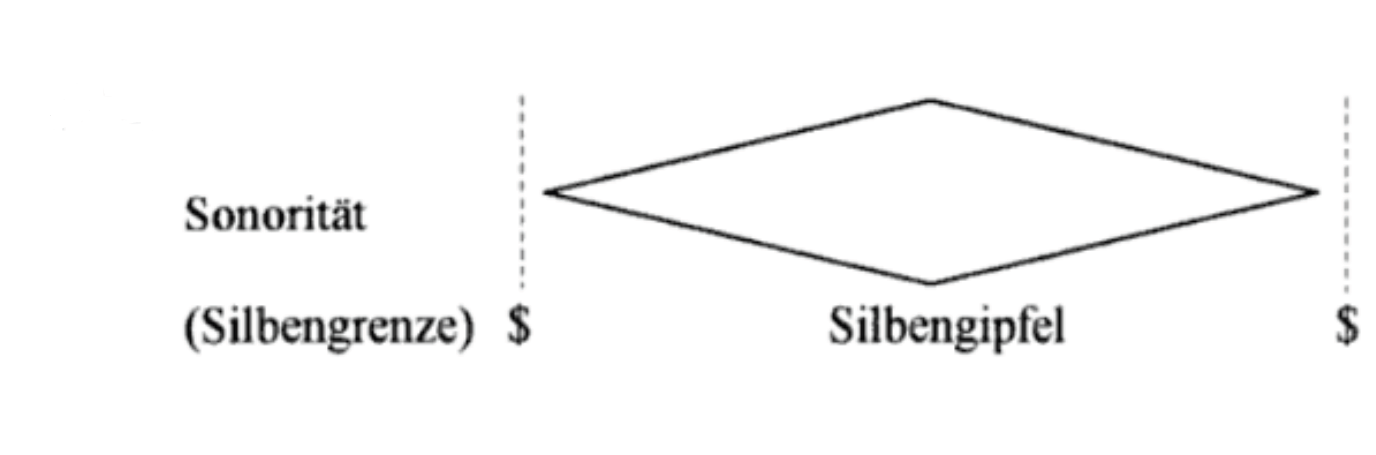
\includegraphics[scale=.2]{../material/03bSonoritaetRamers}
\caption{Nach \citet[93]{Ramers08a} (apud Lenerz 1985)}
\end{figure}

\begin{itemize}
	\item Laute können nach der Sonoritätshierarchie auf einer Skala (nach ihrer \textbf{Sonorität}) angeordnet werden.
\end{itemize}

\end{frame}



%%%%%%%%%%%%%%%%%%%%%%%%%%%%%%%%%%

\begin{frame}
\frametitle{Sonoritätshierarchie}

\begin{itemize}
	\item Es gibt verschiedene Ausformulierungen der Sonoritätshierachie.

\end{itemize}

\begin{table}
\centering
\begin{tabular}{l|l|l|l|l} 
	 & einfach 				  	 & Hall 					  & \textbf{Wiese} 				& komplex  \\ 
\hline
\hline 
$[+]$& \multirow{6}{*}{Sonorant} & \multirow{2}{*}{Vokal} 	  & \multirow{2}{*}{Vokal} 		& Vokal  \\ 
	 & 							 & 						 	  &								& Vokal (hoch) \\
\cline{3-5}			
	 &							 & \multirow{3}{*}{Liquide}   &								& Gleitlaut \\
	 &						  	 &	 						  & \textipa{/\textscr /}		& Vibrant \\
\cline{4-5}			
	 &						 	 &							  & \textipa{/l/}				& Lateral \\
\cline{3-5}			
	 &							 & Nasal					  & Nasal						& Nasal \\
\hline			
	 &\multirow{6}{*}{Obstruent} & \multirow{6}{*}{Obstruent} & \multirow{3}{*}{Frikativ}	& $[+$sth$]$ Frikativ \\
	 &						 	 &							  &								& $[+$sth$]$ Affrikat \\		
	 &							 &							  &								& $[+$sth$]$ Plosiv \\
\cline{4-5}			
	 &						  	 &							  & \multirow{3}{*}{Plosiv}		& $[-$sth$]$ Frikativ \\
	 &						 	 &							  &								& $[-$sth$]$ Affrikat \\		
$[-]$&							 &							  &								& $[-$sth$]$ Plosiv \\
		
\end{tabular} 

\end{table}

\end{frame}



%%%%%%%%%%%%%%%%%%%%%%%%%%%%%%%%%%

\begin{frame}
\frametitle{Sonoritätshierarchie}


\begin{block}{Sonoritätsprinzip (Sonority Sequencing Generalization -- SSG)}
In jeder Silbe gibt es ein Segment, das den Silbengipfel bildet, und dem ein oder mehrere Segmente vorangehen und/oder folgen, deren Sonoritätswerte zum Silbengipfel hin zunehmen und danach abnehmen. (vgl. \citealt[225]{Hall00a}, \citealt[94]{Ramers08a})
\end{block}

\begin{itemize}
	\item Strikt: Monoton steigend oder fallend
	\item Abgeschwächt: auch gleichbleibend \citep[vgl.][]{Hall00a}

\end{itemize}

\begin{figure}
\centering
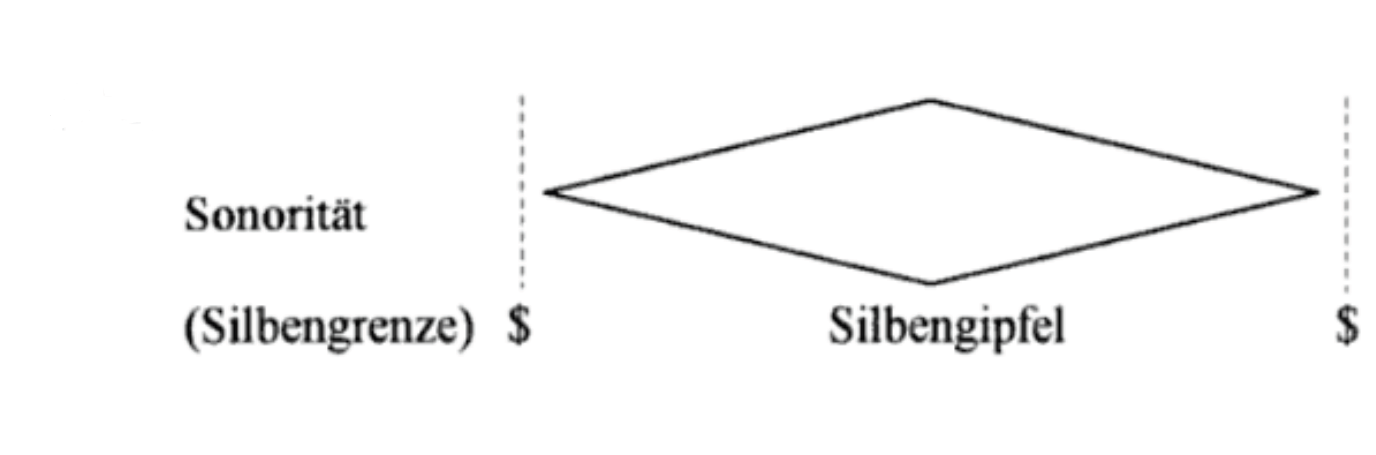
\includegraphics[scale=.2]{../material/03bSonoritaetRamers}
\caption{Nach \citet[93]{Ramers08a} (apud Lenerz 1985)}
\end{figure}

\end{frame}



%%%%%%%%%%%%%%%%%%%%%%%%%%%%%%%%%%

\begin{frame}
\frametitle{Sonoritätshierarchie}

\begin{block}{Sonoritätshierarchie (für uns)}
Vokal $>$ \textipa{/\textscr /} $>$ \textipa{/l/} $>$ Nasal $>$ Frikativ $>$ Plosiv \\
$x > y$ $:=$ $x$ ist sonorer als $y$
\end{block}


\begin{figure}
\centering
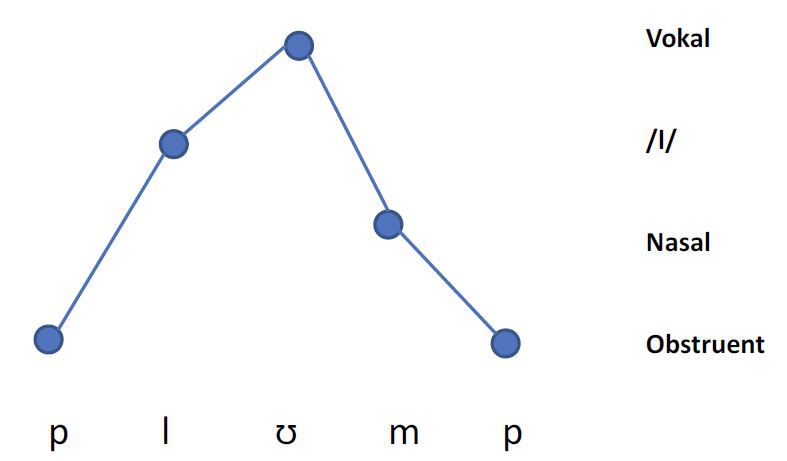
\includegraphics[scale=.3]{../material/03bSonoritaetBsp}
\caption{Nach \citet[225]{Hall00a}}
\end{figure}

\begin{itemize}
	\item Sonoritätshierarchie wird je nach Sprache leicht anders spezifiziert.
\end{itemize}
\end{frame}



%%%%%%%%%%%%%%%%%%%%%%%%%%%%%%%%%%
\begin{frame}
\frametitle{Sonoritätshierarchie}

\begin{itemize}
	\item Geben Sie die Sonoritätsprofile der folgenden Silben an.
	
	\ex. Spatz, Dachs, Clown, Milch

	\item Erklären Sie die Ungramatikalität der folgenden Silben:
	
	\ex. *\textipa{[lbat]}, *\textipa{[\textscr to:k]}, *\textipa{[nki:l]}, *\textipa{[ngak]}

	\ex. *\textipa{[katl]}, *\textipa{[hat\textscr ]}, *\textipa{[latn]}, *\textipa{[k\textscr akN]}

\end{itemize}

\end{frame}



%%%%%%%%%%%%%%%%%%%%%%%%%%%%%%%%%%
%%%%%%%%%%%%%%%%%%%%%%%%%%%%%%%%%%
\subsection{Weitere phonotaktische Beschränkungen}
%\frame{
%\frametitle{~}
%\begin{multicols}{2}
%	\tableofcontents[currentsection]
%\end{multicols}	
%}
%%%%%%%%%%%%%%%%%%%%%%%%%%%%%%%%%%

\begin{frame}
\frametitle{Weitere phonotaktische Beschränkungen}

\begin{itemize}
	\item Im \textbf{Onset} in deutschen Silben können stehen:

	\begin{itemize}
		\item alle Einzelkonsonanten des Deutschen,
		\item außer \textipa{[s]} vor V, und \textipa{[N]}
		\item[]
		\item bestimmte zwei- und dreigliedrige Konsonantencluster (nach Sonoritätshierarchie)
	\end{itemize}
	
	\item[]

	\item Silben können auch \textbf{mit unbetontem Vokal} beginnen.

	\begin{itemize}
		\item Dann ist der Onset leer.
		\ex. \textipa{[\textprimstress PaI.5]} 

		\ex. \textipa{[PEt.\textprimstress va:.I\c{c}]}
	
	\end{itemize}
	
	\item Vor betontem Vokal steht immer der \textbf{Glottisschlag}.

	\ex. \textipa{[ka.\textprimstress Po:.tIS]}

\end{itemize}

\end{frame}



%%%%%%%%%%%%%%%%%%%%%%%%%%%%%%%%%%
%%%%%%%%%%%%%%%%%%%%%%%%%%%%%%%%%%
\section{Silbenmodelle}
\frame{
\frametitle{~}
\begin{multicols}{2}
	\tableofcontents[currentsection]
\end{multicols}	

}
%%%%%%%%%%%%%%%%%%%%%%%%%%%%%%%%%%

\begin{frame}
\frametitle{Silbenmodelle}

\begin{itemize}
	\item Bisher (hauptsächlich) nur \textbf{lineare Betrachtung} mit allen Segmenten auf einer Schicht
	\ex. \textipa{/pe:.t@\textscr /}
	
	\ex. \textipa{/vE\.t@\textscr /}

	\item \textbf{Nicht-lineare Phonologie} (Autosegmentale Phonologie)
	
	\begin{itemize}
		\item verschiedene Repräsentationsebenen bzw. Schichten
		
		\item hierarchische Strukturierung
		
		\item Vorteil: Beschreibung von \textbf{Merkmalsausbreitung} und \textbf{segmentunabhängigen Prozessen}
		
	\end{itemize}
\end{itemize}

\end{frame}



%%%%%%%%%%%%%%%%%%%%%%%%%%%%%%%%%%
%%%%%%%%%%%%%%%%%%%%%%%%%%%%%%%%%%
\subsection{CV-Modell}
%\frame{
%\frametitle{~}
%	\tableofcontents[currentsection]
%}


%%%%%%%%%%%%%%%%%%%%%%%%%%%%%%%%%%
\begin{frame}
\frametitle{CV-Modell (Einfaches Modell)}

\begin{itemize}
	\item Silben und Segmente auf unterschiedlichen Schichten
		
	\item Verbunden durch Assoziationslinien
		
	\item Charakterisierung der Silbenstruktur durch C und V 
\end{itemize}


\begin{figure}
\centering
\begin{forest}
sn edges,
[$\sigma$
	[C [\textipa{b}]]
	[C [\textipa{l}]]
	[V [\textipa{I}]]
	[C [\textipa{n}]]
	[C [\textipa{t}]]
]
\end{forest}
\caption{CV-Modell}
\end{figure}


\begin{itemize}
		\item $\sigma :=$ Silbe
		\item C $:=$ nicht-silbisch, konsonantisch
		\item V $:=$ silbisch, vokalisch
\end{itemize}

\end{frame}



%%%%%%%%%%%%%%%%%%%%%%%%%%%%%%%%%%

\begin{frame}
\frametitle{CV-Modell (Einfaches Modell)}

\begin{itemize}
	\item Wie ist die Verteilung von Segmenten in der Silbe (im Deutschen)?
\end{itemize}

\begin{minipage}{.59\textwidth}
\begin{itemize}
	\item C $\neq$ Konsonant, sondern \textbf{nicht-silbisch}
	\item[]
	\item V $\neq$ Vokal, sondern \textbf{silbisch}
	\item[]
	\item Jede Silbe enthält einen \textbf{Kern} (V)
\end{itemize}
\end{minipage}
%
\begin{minipage}{.4\textwidth}

\begin{figure}
%\tiny
\small
\centering
\begin{forest}
sn edges,
[$\sigma$
	[C [\textipa{g}]]
	[C [\textipa{l}]]
	[V [\textipa{a}]]	
	[C [\textipa{U}]]
	[C [\textipa{p}]]
	[C [\textipa{t}]]
]
\end{forest}

\begin{forest}
sn edges,
[$\sigma$
	[C [\textipa{k}]]
	[V [\textipa{U}]]
	[C [\textipa{m}]]	
]
\end{forest}
%
\begin{forest}
sn edges,
[$\sigma$
	[C [\textipa{p}]]
	[V [\textipa{\textsyllabic{l}}]]
]
\end{forest}

\end{figure}

\end{minipage}

\end{frame}



%%%%%%%%%%%%%%%%%%%%%%%%%%%%%%%%%%

\begin{frame}
\frametitle{CV-Modell (Einfaches Modell)}

\begin{itemize}
	\item Wie ist die Verteilung von Segmenten in der Silbe (im Deutschen)?
\end{itemize}

\begin{minipage}{.59\textwidth}
\begin{itemize}
	\item \textbf{Maximale Anzahl an Cs} vor und nach V
	\item[]
	\item Korrelation zwischen Anzahl an Cs nach V und der \textbf{Länge}/(Un-)Gespanntheit des Vokals
\end{itemize}
\end{minipage}
%
\begin{minipage}{.4\textwidth}

\begin{figure}
%\tiny
\small
\centering
\begin{forest}
sn edges,
[$\sigma$
	[C [\textipa{g}]]
	[C [\textipa{l}]]
	[V [\textipa{a}]]	
	[C [\textipa{U}]]
	[C [\textipa{p}]]
	[C [\textipa{t}]]
]
\end{forest}

\begin{forest}
sn edges,
[$\sigma$
	[C [\textipa{k}]]
	[C [\textipa{\textscr }]]
	[V [\textipa{a}]]
	[C [\textipa{N}]]
	[C [\textipa{k}]]	
]
\end{forest}

\end{figure}

\end{minipage}

\end{frame}



%%%%%%%%%%%%%%%%%%%%%%%%%%%%%%%%%%

\begin{frame}
\frametitle{CV-Modell (Einfaches Modell)}

\begin{itemize}
	\item Wie ist die Verteilung von Segmenten in der Silbe (im Deutschen)?
\end{itemize}

\begin{minipage}{.59\textwidth}
\begin{itemize}
	\item Diphthonge \ras VC (bzw. CV \textipa{[g\textsubarch{U}Ot]})
	\item[]
	\item Lange Vokale \ras VC
	\item[]
	\item Affrikate \ras C
	\item[]
	\item Silbische Konsonanten \ras V
\end{itemize}
\end{minipage}
%
\begin{minipage}{.4\textwidth}

\begin{figure}
\tiny
%\scriptsize
\centering
\begin{forest}
sn edges,
[$\sigma$
	[C [\textipa{g}]]
	[C [\textipa{l}]]
	[V [\textipa{a}]]	
	[C [\textipa{U}]]
	[C [\textipa{p}]]
	[C [\textipa{t}]]
]
\end{forest}

\begin{forest}
sn edges,
[$\sigma$
	[C [\textipa{k}]]
	[V [\textipa{a}]]
	[C [\textipa{:}]]	
	[C [\textipa{l}]]
]
\end{forest}

\begin{forest}
sn edges,
[$\sigma$
	[C [\textipa{k}]]
	[V [\textipa{O}]]
	[C [\textipa{\t{pf}}]]	
	[C [\textipa{s}]]
]
\end{forest}

\begin{forest}
sn edges,
[$\sigma$
	[C [\textipa{k}]]
	[V [\textipa{U}]]
	[C [\textipa{m}]]	
]
\end{forest}
%
\begin{forest}
sn edges,
[$\sigma$
	[C [\textipa{p}]]
	[V [\textipa{\textsyllabic{l}}]]
]
\end{forest}

\end{figure}

\end{minipage}

\end{frame}



%%%%%%%%%%%%%%%%%%%%%%%%%%%%%%%%%%
%%%%%%%%%%%%%%%%%%%%%%%%%%%%%%%%%%
\subsection{Konstituentenmodell}
%\frame{
%\begin{multicols}{2}
%\frametitle{~}
%	\tableofcontents[currentsection]
%\end{multicols}
%}
%%%%%%%%%%%%%%%%%%%%%%%%%%%%%%%%%%

\begin{frame}
\frametitle{Konstituentenmodell}

\begin{itemize}
	\item Zerlegung in \textbf{silbische Konstituenten}
	\item Silbe ($\sigma$) = Onset (O) + Reim (R)
	\item Reim (R) = Nukleus (N) + Koda (K)
	\item + Skelettschicht (X)
\end{itemize}


\begin{figure}
%%%%%%%%%%%%%
%%% Forestset Syllables

\newbox\foreststrutbox
\setbox\foreststrutbox=\hbox to 0pt{\phantom{\forestOve{standard node}{content}}}
\def\foreststrut{\copy\foreststrutbox}
\forestset{
GP1/.style 2 args={
for n={1}{baseline},
s sep=0pt, l sep=0pt,
for descendants={
l sep=0pt, l={#1},
anchor=base,calign=first,child anchor=north,
inner xsep=1pt,inner ysep=2pt,outer sep=0pt,s sep=0pt,
},
delay={
if content={}{phantom}{for children={no edge}},
for tree={
if content={O}{tier=OR}{},
if content={R}{tier=OR}{},
if content={N}{tier=N}{},
if content={x}{
tier=x,content={$\times$},outer xsep={#2},
for tree={calign=center},
for descendants={content format={\foreststrut\forestoption{content}}},
before drawing tree={outer xsep=0pt,delay={typeset node}},
s sep=4pt
}{},
},
},
before drawing tree={where content={}{parent anchor=center,child anchor=center}{}},
},
GP1/.default={5ex}{8.0pt},
associate/.style={%
tikz+={\draw(!)--(!#1);}},
spread/.style={
before drawing tree={tikz+={\draw[dotted](!)--(!#1);}}},
govern/.style={
before drawing tree={tikz+={\draw[->](!)--(!#1);}}},
p-govern/.style={
before drawing tree={tikz+={\draw[->](.north) to[out=150,in=30] (!#1.north);}}},
no p-govern/.style={
before drawing tree={tikz+={\draw[->,loosely dashed](.north) to[out=150,in=30] (!#1.north);}}},
encircle/.style={before drawing tree={circle,draw,inner sep=0pt}},
fen/.style={pin={[font=\footnotesize,inner sep=1pt,pin edge=<-]10:\textsc{Fen}}},
el/.style={content=\textsc{\textbf{##1}}},
head/.style={content=\textsc{\textbf{\underline{##1}}}},
llap/.style={
tikz+={%
\edef\forest@temp{\noexpand\node[\option{node options},
anchor=base east,at=(.base east)]}%
\forest@temp{#1\phantom{\option{environment}}};
}
},
rlap/.style={
tikz+={%
\edef\forest@temp{\noexpand\node[\option{node options},
anchor=base west,at=(.base west)]}%
\forest@temp{\phantom{\option{environment}}#1};
}
},
}
%%%%%%%%%%%%%

\small
\centering
\begin{forest} sn edges, GP1 [
  [$\sigma$
    [O[x[\textipa{f}]][x[\textipa{K}]]]
    [R[N[x[\textipa{\textopeno}]]][K[x[\textipa{s}]]]]
  ]
  [$\sigma$
    [O[x[\textipa{t}]]]
    [R[N[x[\textipa{I}]]][K[x[\c{c}]]]]
  ]  
]
\end{forest}

\caption{Konstituentenmodell}
\end{figure}

\end{frame}



%%%%%%%%%%%%%%%%%%%%%%%%%%%%%%%%%%

\begin{frame}
\frametitle{Konstituentenmodell}

\textbf{Silbe} ($\sigma$) = Onset (O) + Reim (R)

\begin{itemize}
	\item \textbf{Onset}: 
	\begin{itemize}
		\item Versprecher
	
	\ex. \textipa{kIl\c{c}.ma\.f@} vs. \textipa{mIl\c{c}.ka\.f@}

	\end{itemize}	
			
	\item \textbf{Reim}: 
	\begin{itemize}
		\item Silbengewicht: Längenausgleich zwischen N und K 		
		\item Gedichte
		\item Typischerweise VCC oder VVC
	\end{itemize}
	
\end{itemize}

\textbf{Reim} (R) = Nukleus (N) + Koda (K)

\begin{itemize}
	\item \textbf{Nukleus}: 
	\begin{itemize}
		\item Obligatorisch
	\end{itemize}	
			
	\item \textbf{Koda}: 
	\begin{itemize}
		\item Regeln, die sich nur auf die Konsonanten in der Koda beziehen
	\end{itemize}
	
\end{itemize}

\end{frame}



%%%%%%%%%%%%%%%%%%%%%%%%%%%%%%%%%

\begin{frame}
\frametitle{Konstituentenmodell}

\textbf{Skelettschicht}

\begin{itemize}
	\item Ebene zwischen den Segmenten und den Silbenkonstituenten
	
	\item X $:=$ abstrakte Zeiteinheit (\zB für Darstellung des Längenausgleichs)
	
	\item X \ras Vergleichbar mit C und V

	\item \textbf{Nukleus}:
	
	\begin{itemize}
		\item 1 X: Kurzvokal
		\item 2 X: Langvokal, Diphthong
		\item (3 X: Langvokal + vokalisiertes \textipa{/\textscr /})
	\end{itemize}
	
\end{itemize}


\begin{minipage}{.325\textwidth}

%%%%%%%%%%%%%
%%% Forestset Syllables

\newbox\foreststrutbox
\setbox\foreststrutbox=\hbox to 0pt{\phantom{\forestOve{standard node}{content}}}
\def\foreststrut{\copy\foreststrutbox}
\forestset{
GP1/.style 2 args={
for n={1}{baseline},
s sep=0pt, l sep=0pt,
for descendants={
l sep=0pt, l={#1},
anchor=base,calign=first,child anchor=north,
inner xsep=1pt,inner ysep=2pt,outer sep=0pt,s sep=0pt,
},
delay={
if content={}{phantom}{for children={no edge}},
for tree={
if content={O}{tier=OR}{},
if content={R}{tier=OR}{},
if content={N}{tier=N}{},
if content={x}{
tier=x,content={$\times$},outer xsep={#2},
for tree={calign=center},
for descendants={content format={\foreststrut\forestoption{content}}},
before drawing tree={outer xsep=0pt,delay={typeset node}},
s sep=4pt
}{},
},
},
before drawing tree={where content={}{parent anchor=center,child anchor=center}{}},
},
GP1/.default={5ex}{8.0pt},
associate/.style={%
tikz+={\draw(!)--(!#1);}},
spread/.style={
before drawing tree={tikz+={\draw[dotted](!)--(!#1);}}},
govern/.style={
before drawing tree={tikz+={\draw[->](!)--(!#1);}}},
p-govern/.style={
before drawing tree={tikz+={\draw[->](.north) to[out=150,in=30] (!#1.north);}}},
no p-govern/.style={
before drawing tree={tikz+={\draw[->,loosely dashed](.north) to[out=150,in=30] (!#1.north);}}},
encircle/.style={before drawing tree={circle,draw,inner sep=0pt}},
fen/.style={pin={[font=\footnotesize,inner sep=1pt,pin edge=<-]10:\textsc{Fen}}},
el/.style={content=\textsc{\textbf{##1}}},
head/.style={content=\textsc{\textbf{\underline{##1}}}},
llap/.style={
tikz+={%
\edef\forest@temp{\noexpand\node[\option{node options},
anchor=base east,at=(.base east)]}%
\forest@temp{#1\phantom{\option{environment}}};
}
},
rlap/.style={
tikz+={%
\edef\forest@temp{\noexpand\node[\option{node options},
anchor=base west,at=(.base west)]}%
\forest@temp{\phantom{\option{environment}}#1};
}
},
}
%%%%%%%%%%%%%

\small
\centering
\begin{forest} sn edges, GP1 [
  [$\sigma$
    [O[x[\textipa{m}]]]
    [R[N[x[\textipa{I}]]][K[x[t]]]]
  ]  
]
\end{forest}

\end{minipage}
%
\begin{minipage}{.325\textwidth}
%%%%%%%%%%%%%
%%% Forestset Syllables

\newbox\foreststrutbox
\setbox\foreststrutbox=\hbox to 0pt{\phantom{\forestOve{standard node}{content}}}
\def\foreststrut{\copy\foreststrutbox}
\forestset{
GP1/.style 2 args={
for n={1}{baseline},
s sep=0pt, l sep=0pt,
for descendants={
l sep=0pt, l={#1},
anchor=base,calign=first,child anchor=north,
inner xsep=1pt,inner ysep=2pt,outer sep=0pt,s sep=0pt,
},
delay={
if content={}{phantom}{for children={no edge}},
for tree={
if content={O}{tier=OR}{},
if content={R}{tier=OR}{},
if content={N}{tier=N}{},
if content={x}{
tier=x,content={$\times$},outer xsep={#2},
for tree={calign=center},
for descendants={content format={\foreststrut\forestoption{content}}},
before drawing tree={outer xsep=0pt,delay={typeset node}},
s sep=4pt
}{},
},
},
before drawing tree={where content={}{parent anchor=center,child anchor=center}{}},
},
GP1/.default={5ex}{8.0pt},
associate/.style={%
tikz+={\draw(!)--(!#1);}},
spread/.style={
before drawing tree={tikz+={\draw[dotted](!)--(!#1);}}},
govern/.style={
before drawing tree={tikz+={\draw[->](!)--(!#1);}}},
p-govern/.style={
before drawing tree={tikz+={\draw[->](.north) to[out=150,in=30] (!#1.north);}}},
no p-govern/.style={
before drawing tree={tikz+={\draw[->,loosely dashed](.north) to[out=150,in=30] (!#1.north);}}},
encircle/.style={before drawing tree={circle,draw,inner sep=0pt}},
fen/.style={pin={[font=\footnotesize,inner sep=1pt,pin edge=<-]10:\textsc{Fen}}},
el/.style={content=\textsc{\textbf{##1}}},
head/.style={content=\textsc{\textbf{\underline{##1}}}},
llap/.style={
tikz+={%
\edef\forest@temp{\noexpand\node[\option{node options},
anchor=base east,at=(.base east)]}%
\forest@temp{#1\phantom{\option{environment}}};
}
},
rlap/.style={
tikz+={%
\edef\forest@temp{\noexpand\node[\option{node options},
anchor=base west,at=(.base west)]}%
\forest@temp{\phantom{\option{environment}}#1};
}
},
}
%%%%%%%%%%%%%

\small
\centering
\begin{forest} sn edges, GP1 [
  [$\sigma$
    [O[x[\textipa{z}]]]
    [R
    	[N
    		[x
    			[\textipa{e:}]
    		]
    		[x]{\draw[black] (.south)--++(-2.38em,-2.3ex);}
    	]
    	[K []]]
  ]  
]
\end{forest}

\end{minipage}
%
\begin{minipage}{.325\textwidth}
%%%%%%%%%%%%%
%%% Forestset Syllables

\newbox\foreststrutbox
\setbox\foreststrutbox=\hbox to 0pt{\phantom{\forestOve{standard node}{content}}}
\def\foreststrut{\copy\foreststrutbox}
\forestset{
GP1/.style 2 args={
for n={1}{baseline},
s sep=0pt, l sep=0pt,
for descendants={
l sep=0pt, l={#1},
anchor=base,calign=first,child anchor=north,
inner xsep=1pt,inner ysep=2pt,outer sep=0pt,s sep=0pt,
},
delay={
if content={}{phantom}{for children={no edge}},
for tree={
if content={O}{tier=OR}{},
if content={R}{tier=OR}{},
if content={N}{tier=N}{},
if content={x}{
tier=x,content={$\times$},outer xsep={#2},
for tree={calign=center},
for descendants={content format={\foreststrut\forestoption{content}}},
before drawing tree={outer xsep=0pt,delay={typeset node}},
s sep=4pt
}{},
},
},
before drawing tree={where content={}{parent anchor=center,child anchor=center}{}},
},
GP1/.default={5ex}{8.0pt},
associate/.style={%
tikz+={\draw(!)--(!#1);}},
spread/.style={
before drawing tree={tikz+={\draw[dotted](!)--(!#1);}}},
govern/.style={
before drawing tree={tikz+={\draw[->](!)--(!#1);}}},
p-govern/.style={
before drawing tree={tikz+={\draw[->](.north) to[out=150,in=30] (!#1.north);}}},
no p-govern/.style={
before drawing tree={tikz+={\draw[->,loosely dashed](.north) to[out=150,in=30] (!#1.north);}}},
encircle/.style={before drawing tree={circle,draw,inner sep=0pt}},
fen/.style={pin={[font=\footnotesize,inner sep=1pt,pin edge=<-]10:\textsc{Fen}}},
el/.style={content=\textsc{\textbf{##1}}},
head/.style={content=\textsc{\textbf{\underline{##1}}}},
llap/.style={
tikz+={%
\edef\forest@temp{\noexpand\node[\option{node options},
anchor=base east,at=(.base east)]}%
\forest@temp{#1\phantom{\option{environment}}};
}
},
rlap/.style={
tikz+={%
\edef\forest@temp{\noexpand\node[\option{node options},
anchor=base west,at=(.base west)]}%
\forest@temp{\phantom{\option{environment}}#1};
}
},
}
%%%%%%%%%%%%%

\small
\centering
\begin{forest} sn edges, GP1 [
  [$\sigma$
    [O[x[\textipa{P}]]]
    [R
    	[N
    		[x
    			[\textipa{\t{aU}}]
    		]
    		[x]{\draw[black] (.south)--++(-2.38em,-1.7ex);}
    	]
    	[K[x[\textipa{x}]]]]
  ]  
]
\end{forest}

\end{minipage}

\end{frame}



%%%%%%%%%%%%%%%%%%%%%%%%%%%%%%%%%

\begin{frame}
\frametitle{Konstituentenmodell}

\textbf{Skelettschicht}

\begin{itemize}

	\item \textbf{Onset} und \textbf{Koda}:
	
	\begin{itemize}
		\item Pro C ein X
		\item Ausnahme: Affrikate \ras 1 X (Eine Zeiteinheit!)
		\item Ausnahme: Silbengelenk (s.u.)
	
	\end{itemize}
\end{itemize}

\begin{minipage}{.3\textwidth}
%%%%%%%%%%%%%
%%% Forestset Syllables

\newbox\foreststrutbox
\setbox\foreststrutbox=\hbox to 0pt{\phantom{\forestOve{standard node}{content}}}
\def\foreststrut{\copy\foreststrutbox}
\forestset{
GP1/.style 2 args={
for n={1}{baseline},
s sep=0pt, l sep=0pt,
for descendants={
l sep=0pt, l={#1},
anchor=base,calign=first,child anchor=north,
inner xsep=1pt,inner ysep=2pt,outer sep=0pt,s sep=0pt,
},
delay={
if content={}{phantom}{for children={no edge}},
for tree={
if content={O}{tier=OR}{},
if content={R}{tier=OR}{},
if content={N}{tier=N}{},
if content={x}{
tier=x,content={$\times$},outer xsep={#2},
for tree={calign=center},
for descendants={content format={\foreststrut\forestoption{content}}},
before drawing tree={outer xsep=0pt,delay={typeset node}},
s sep=4pt
}{},
},
},
before drawing tree={where content={}{parent anchor=center,child anchor=center}{}},
},
GP1/.default={5ex}{8.0pt},
associate/.style={%
tikz+={\draw(!)--(!#1);}},
spread/.style={
before drawing tree={tikz+={\draw[dotted](!)--(!#1);}}},
govern/.style={
before drawing tree={tikz+={\draw[->](!)--(!#1);}}},
p-govern/.style={
before drawing tree={tikz+={\draw[->](.north) to[out=150,in=30] (!#1.north);}}},
no p-govern/.style={
before drawing tree={tikz+={\draw[->,loosely dashed](.north) to[out=150,in=30] (!#1.north);}}},
encircle/.style={before drawing tree={circle,draw,inner sep=0pt}},
fen/.style={pin={[font=\footnotesize,inner sep=1pt,pin edge=<-]10:\textsc{Fen}}},
el/.style={content=\textsc{\textbf{##1}}},
head/.style={content=\textsc{\textbf{\underline{##1}}}},
llap/.style={
tikz+={%
\edef\forest@temp{\noexpand\node[\option{node options},
anchor=base east,at=(.base east)]}%
\forest@temp{#1\phantom{\option{environment}}};
}
},
rlap/.style={
tikz+={%
\edef\forest@temp{\noexpand\node[\option{node options},
anchor=base west,at=(.base west)]}%
\forest@temp{\phantom{\option{environment}}#1};
}
},
}
%%%%%%%%%%%%%

\footnotesize
\centering
\begin{forest} sn edges, GP1 [
  [$\sigma$
    [O
    	[x[\textipa{f}]]
    	[x[\textipa{\textscr }]]
    ]
    [R
    	[N
    		[x
    			[\textipa{E}]
    		]
    	]
    	[K [x[\textipa{\c{c}}]]]]
  ]  
]
\end{forest}

\end{minipage}
%
\begin{minipage}{.28\textwidth}

%%%%%%%%%%%%%
%%% Forestset Syllables

\newbox\foreststrutbox
\setbox\foreststrutbox=\hbox to 0pt{\phantom{\forestOve{standard node}{content}}}
\def\foreststrut{\copy\foreststrutbox}
\forestset{
GP1/.style 2 args={
for n={1}{baseline},
s sep=0pt, l sep=0pt,
for descendants={
l sep=0pt, l={#1},
anchor=base,calign=first,child anchor=north,
inner xsep=1pt,inner ysep=2pt,outer sep=0pt,s sep=0pt,
},
delay={
if content={}{phantom}{for children={no edge}},
for tree={
if content={O}{tier=OR}{},
if content={R}{tier=OR}{},
if content={N}{tier=N}{},
if content={x}{
tier=x,content={$\times$},outer xsep={#2},
for tree={calign=center},
for descendants={content format={\foreststrut\forestoption{content}}},
before drawing tree={outer xsep=0pt,delay={typeset node}},
s sep=4pt
}{},
},
},
before drawing tree={where content={}{parent anchor=center,child anchor=center}{}},
},
GP1/.default={5ex}{8.0pt},
associate/.style={%
tikz+={\draw(!)--(!#1);}},
spread/.style={
before drawing tree={tikz+={\draw[dotted](!)--(!#1);}}},
govern/.style={
before drawing tree={tikz+={\draw[->](!)--(!#1);}}},
p-govern/.style={
before drawing tree={tikz+={\draw[->](.north) to[out=150,in=30] (!#1.north);}}},
no p-govern/.style={
before drawing tree={tikz+={\draw[->,loosely dashed](.north) to[out=150,in=30] (!#1.north);}}},
encircle/.style={before drawing tree={circle,draw,inner sep=0pt}},
fen/.style={pin={[font=\footnotesize,inner sep=1pt,pin edge=<-]10:\textsc{Fen}}},
el/.style={content=\textsc{\textbf{##1}}},
head/.style={content=\textsc{\textbf{\underline{##1}}}},
llap/.style={
tikz+={%
\edef\forest@temp{\noexpand\node[\option{node options},
anchor=base east,at=(.base east)]}%
\forest@temp{#1\phantom{\option{environment}}};
}
},
rlap/.style={
tikz+={%
\edef\forest@temp{\noexpand\node[\option{node options},
anchor=base west,at=(.base west)]}%
\forest@temp{\phantom{\option{environment}}#1};
}
},
}
%%%%%%%%%%%%%

\footnotesize
\centering
\begin{forest} sn edges, GP1 [
  [$\sigma$
    [O[x[\textipa{k}]]]
    [R[N[x[\textipa{O}]]][K[x[\textipa{\t{pf}}]]]]
  ]  
]
\end{forest}

\end{minipage}
%
\begin{minipage}{.35\textwidth}
%%%%%%%%%%%%%
%%% Forestset Syllables

\newbox\foreststrutbox
\setbox\foreststrutbox=\hbox to 0pt{\phantom{\forestOve{standard node}{content}}}
\def\foreststrut{\copy\foreststrutbox}
\forestset{
GP1/.style 2 args={
for n={1}{baseline},
s sep=0pt, l sep=0pt,
for descendants={
l sep=0pt, l={#1},
anchor=base,calign=first,child anchor=north,
inner xsep=1pt,inner ysep=2pt,outer sep=0pt,s sep=0pt,
},
delay={
if content={}{phantom}{for children={no edge}},
for tree={
if content={O}{tier=OR}{},
if content={R}{tier=OR}{},
if content={N}{tier=N}{},
if content={x}{
tier=x,content={$\times$},outer xsep={#2},
for tree={calign=center},
for descendants={content format={\foreststrut\forestoption{content}}},
before drawing tree={outer xsep=0pt,delay={typeset node}},
s sep=4pt
}{},
},
},
before drawing tree={where content={}{parent anchor=center,child anchor=center}{}},
},
GP1/.default={5ex}{8.0pt},
associate/.style={%
tikz+={\draw(!)--(!#1);}},
spread/.style={
before drawing tree={tikz+={\draw[dotted](!)--(!#1);}}},
govern/.style={
before drawing tree={tikz+={\draw[->](!)--(!#1);}}},
p-govern/.style={
before drawing tree={tikz+={\draw[->](.north) to[out=150,in=30] (!#1.north);}}},
no p-govern/.style={
before drawing tree={tikz+={\draw[->,loosely dashed](.north) to[out=150,in=30] (!#1.north);}}},
encircle/.style={before drawing tree={circle,draw,inner sep=0pt}},
fen/.style={pin={[font=\footnotesize,inner sep=1pt,pin edge=<-]10:\textsc{Fen}}},
el/.style={content=\textsc{\textbf{##1}}},
head/.style={content=\textsc{\textbf{\underline{##1}}}},
llap/.style={
tikz+={%
\edef\forest@temp{\noexpand\node[\option{node options},
anchor=base east,at=(.base east)]}%
\forest@temp{#1\phantom{\option{environment}}};
}
},
rlap/.style={
tikz+={%
\edef\forest@temp{\noexpand\node[\option{node options},
anchor=base west,at=(.base west)]}%
\forest@temp{\phantom{\option{environment}}#1};
}
},
}
%%%%%%%%%%%%%

\footnotesize
\centering
\begin{forest} sn edges, GP1 [
  [$\sigma$
    [O
    	[x
    		[\textipa{m}]
    	]
    ]
    [R
    	[N
    		[x
    			[\textipa{I}]
    		]
    	]  		
    	[K 
    		[x
    			[\textipa{t}]
    		]
    	]
    ]
  ]
  [$\sigma$
    [O 
    ]{\draw[black] (.south)--++(-1.6em,-6.2ex);}
    [R
    	[N
    		[x
    			[\textipa{@}]
    		]
    	]
    	[K [x[\textipa{n}]]]]
  ]  
]
\end{forest}

\end{minipage}

\end{frame}



%%%%%%%%%%%%%%%%%%%%%%%%%%%%%%%%%%%

\begin{frame}
\frametitle{Konstituentenmodell}

Zusammenhang zwischen Vokallänge und Besetzung der Koda \ras Reim

\begin{block}{Lange Vokale}
Nach einem langen Vokal oder einem Diphthong steht in monomorphemischen Silben kein Konsonantencluster. 

Es gibt wenige Ausnahmen: Mond, Obst
\end{block}


\begin{block}{Kurze Vokale}
In betonten Silben folgt auf einen ungespannten (kurzen) Vokal meistens ein Konsonant
\end{block}	


\begin{minipage}{.325\textwidth}
%%%%%%%%%%%%%
%%% Forestset Syllables

\newbox\foreststrutbox
\setbox\foreststrutbox=\hbox to 0pt{\phantom{\forestOve{standard node}{content}}}
\def\foreststrut{\copy\foreststrutbox}
\forestset{
GP1/.style 2 args={
for n={1}{baseline},
s sep=0pt, l sep=0pt,
for descendants={
l sep=0pt, l={#1},
anchor=base,calign=first,child anchor=north,
inner xsep=1pt,inner ysep=2pt,outer sep=0pt,s sep=0pt,
},
delay={
if content={}{phantom}{for children={no edge}},
for tree={
if content={O}{tier=OR}{},
if content={R}{tier=OR}{},
if content={N}{tier=N}{},
if content={x}{
tier=x,content={$\times$},outer xsep={#2},
for tree={calign=center},
for descendants={content format={\foreststrut\forestoption{content}}},
before drawing tree={outer xsep=0pt,delay={typeset node}},
s sep=4pt
}{},
},
},
before drawing tree={where content={}{parent anchor=center,child anchor=center}{}},
},
GP1/.default={5ex}{8.0pt},
associate/.style={%
tikz+={\draw(!)--(!#1);}},
spread/.style={
before drawing tree={tikz+={\draw[dotted](!)--(!#1);}}},
govern/.style={
before drawing tree={tikz+={\draw[->](!)--(!#1);}}},
p-govern/.style={
before drawing tree={tikz+={\draw[->](.north) to[out=150,in=30] (!#1.north);}}},
no p-govern/.style={
before drawing tree={tikz+={\draw[->,loosely dashed](.north) to[out=150,in=30] (!#1.north);}}},
encircle/.style={before drawing tree={circle,draw,inner sep=0pt}},
fen/.style={pin={[font=\footnotesize,inner sep=1pt,pin edge=<-]10:\textsc{Fen}}},
el/.style={content=\textsc{\textbf{##1}}},
head/.style={content=\textsc{\textbf{\underline{##1}}}},
llap/.style={
tikz+={%
\edef\forest@temp{\noexpand\node[\option{node options},
anchor=base east,at=(.base east)]}%
\forest@temp{#1\phantom{\option{environment}}};
}
},
rlap/.style={
tikz+={%
\edef\forest@temp{\noexpand\node[\option{node options},
anchor=base west,at=(.base west)]}%
\forest@temp{\phantom{\option{environment}}#1};
}
},
}
%%%%%%%%%%%%%

\tiny
\centering
\begin{forest} sn edges, GP1 [
  [$\sigma$
    [O[x[\textipa{z}]]]
    [R
    	[N
    		[x
    			[\textipa{e:}]
    		]
    		[x]{\draw[black] (.south)--++(-2.38em,-2.3ex);}
    	]
    	[K []]]
  ]  
]
\end{forest}

\end{minipage}
%
\begin{minipage}{.325\textwidth}
%%%%%%%%%%%%%
%%% Forestset Syllables

\newbox\foreststrutbox
\setbox\foreststrutbox=\hbox to 0pt{\phantom{\forestOve{standard node}{content}}}
\def\foreststrut{\copy\foreststrutbox}
\forestset{
GP1/.style 2 args={
for n={1}{baseline},
s sep=0pt, l sep=0pt,
for descendants={
l sep=0pt, l={#1},
anchor=base,calign=first,child anchor=north,
inner xsep=1pt,inner ysep=2pt,outer sep=0pt,s sep=0pt,
},
delay={
if content={}{phantom}{for children={no edge}},
for tree={
if content={O}{tier=OR}{},
if content={R}{tier=OR}{},
if content={N}{tier=N}{},
if content={x}{
tier=x,content={$\times$},outer xsep={#2},
for tree={calign=center},
for descendants={content format={\foreststrut\forestoption{content}}},
before drawing tree={outer xsep=0pt,delay={typeset node}},
s sep=4pt
}{},
},
},
before drawing tree={where content={}{parent anchor=center,child anchor=center}{}},
},
GP1/.default={5ex}{8.0pt},
associate/.style={%
tikz+={\draw(!)--(!#1);}},
spread/.style={
before drawing tree={tikz+={\draw[dotted](!)--(!#1);}}},
govern/.style={
before drawing tree={tikz+={\draw[->](!)--(!#1);}}},
p-govern/.style={
before drawing tree={tikz+={\draw[->](.north) to[out=150,in=30] (!#1.north);}}},
no p-govern/.style={
before drawing tree={tikz+={\draw[->,loosely dashed](.north) to[out=150,in=30] (!#1.north);}}},
encircle/.style={before drawing tree={circle,draw,inner sep=0pt}},
fen/.style={pin={[font=\footnotesize,inner sep=1pt,pin edge=<-]10:\textsc{Fen}}},
el/.style={content=\textsc{\textbf{##1}}},
head/.style={content=\textsc{\textbf{\underline{##1}}}},
llap/.style={
tikz+={%
\edef\forest@temp{\noexpand\node[\option{node options},
anchor=base east,at=(.base east)]}%
\forest@temp{#1\phantom{\option{environment}}};
}
},
rlap/.style={
tikz+={%
\edef\forest@temp{\noexpand\node[\option{node options},
anchor=base west,at=(.base west)]}%
\forest@temp{\phantom{\option{environment}}#1};
}
},
}
%%%%%%%%%%%%%

\tiny
\centering
\begin{forest} sn edges, GP1 [
  [$\sigma$
    [O[x[\textipa{P}]]]
    [R
    	[N
    		[x
    			[\textipa{\t{aU}}]
    		]
    		[x]{\draw[black] (.south)--++(-2.38em,-1.7ex);}
    	]
    	[K[x[\textipa{x}]]]]
  ]  
]
\end{forest}

\end{minipage}
%
\begin{minipage}{.325\textwidth}

%%%%%%%%%%%%%
%%% Forestset Syllables

\newbox\foreststrutbox
\setbox\foreststrutbox=\hbox to 0pt{\phantom{\forestOve{standard node}{content}}}
\def\foreststrut{\copy\foreststrutbox}
\forestset{
GP1/.style 2 args={
for n={1}{baseline},
s sep=0pt, l sep=0pt,
for descendants={
l sep=0pt, l={#1},
anchor=base,calign=first,child anchor=north,
inner xsep=1pt,inner ysep=2pt,outer sep=0pt,s sep=0pt,
},
delay={
if content={}{phantom}{for children={no edge}},
for tree={
if content={O}{tier=OR}{},
if content={R}{tier=OR}{},
if content={N}{tier=N}{},
if content={x}{
tier=x,content={$\times$},outer xsep={#2},
for tree={calign=center},
for descendants={content format={\foreststrut\forestoption{content}}},
before drawing tree={outer xsep=0pt,delay={typeset node}},
s sep=4pt
}{},
},
},
before drawing tree={where content={}{parent anchor=center,child anchor=center}{}},
},
GP1/.default={5ex}{8.0pt},
associate/.style={%
tikz+={\draw(!)--(!#1);}},
spread/.style={
before drawing tree={tikz+={\draw[dotted](!)--(!#1);}}},
govern/.style={
before drawing tree={tikz+={\draw[->](!)--(!#1);}}},
p-govern/.style={
before drawing tree={tikz+={\draw[->](.north) to[out=150,in=30] (!#1.north);}}},
no p-govern/.style={
before drawing tree={tikz+={\draw[->,loosely dashed](.north) to[out=150,in=30] (!#1.north);}}},
encircle/.style={before drawing tree={circle,draw,inner sep=0pt}},
fen/.style={pin={[font=\footnotesize,inner sep=1pt,pin edge=<-]10:\textsc{Fen}}},
el/.style={content=\textsc{\textbf{##1}}},
head/.style={content=\textsc{\textbf{\underline{##1}}}},
llap/.style={
tikz+={%
\edef\forest@temp{\noexpand\node[\option{node options},
anchor=base east,at=(.base east)]}%
\forest@temp{#1\phantom{\option{environment}}};
}
},
rlap/.style={
tikz+={%
\edef\forest@temp{\noexpand\node[\option{node options},
anchor=base west,at=(.base west)]}%
\forest@temp{\phantom{\option{environment}}#1};
}
},
}
%%%%%%%%%%%%%

\tiny
\centering
\begin{forest} sn edges, GP1 [
  [$\sigma$
    [O[x[\textipa{m}]]]
    [R[N[x[\textipa{I}]]][K[x[t]]]]
  ]  
]
\end{forest}

\end{minipage}

\end{frame}



%%%%%%%%%%%%%%%%%%%%%%%%%%%%%%%%%%
%%%%%%%%%%%%%%%%%%%%%%%%%%%%%%%%%%

\section{Übung}
\frame{
\frametitle{~}
\begin{multicols}{2}
	\tableofcontents[currentsection]
\end{multicols}	

}


%%%%%%%%%%%%%%%%%%%%%%%%%%%%%%%%%%
\begin{frame}
\frametitle{Übung}

Geben Sie eine phonetische Tranksription der folgenden Wörter nach der \gqq{Standardaussprache} an, zeichnen Sie dabei die Silbestruktur nach dem Konstituentenmodell und mit der Skelettschicht, und geben Sie die Sonoritätsprofile an.

\begin{block}{Sonoritätshierarchie (Zur Erinnerung)}
Vokal $>$ \textipa{/\textscr /} $>$ \textipa{/l/} $>$ Nasal $>$ Frikativ $>$ Plosiv \\
$x > y :=$ $x$ ist sonorer als $y$
\end{block}

\ex. 
\a. sprechen
\b. Obst
\b. Brandschutz
\b. Stimmenfang
\b. Abstandshalter
\b. Mittagessen
\b. Bierdeckel


\end{frame}



%%%%%%%%%%%%%%%%%%%%%%%%%%%%%%%%%%
%%%%%%%%%%%%%%%%%%%%%%%%%%%%%%%%%%
\section{Silbengelenk}
\frame{
\frametitle{~}
\begin{multicols}{2}
	\tableofcontents[currentsection]
\end{multicols}	

}
%%%%%%%%%%%%%%%%%%%%%%%%%%%%%%%%%%

\begin{frame}
\frametitle{Silbengelenk}


\begin{minipage}{.63\textwidth}

\begin{itemize}
	\item \textbf{ambisyllabischer Konsonant}
	
	\item[]
	\item Ein Konsonant, der zugleich \textbf{zu zwei Silben} gehört. 
	
	\item[]
	\item Nur \textbf{eine X Position} (nur eine Zeiteinheit, vgl. echte Geminaten)
	
\end{itemize}
\end{minipage}
%
\begin{minipage}{.35\textwidth}
%%%%%%%%%%%%%
%%% Forestset Syllables

\newbox\foreststrutbox
\setbox\foreststrutbox=\hbox to 0pt{\phantom{\forestOve{standard node}{content}}}
\def\foreststrut{\copy\foreststrutbox}
\forestset{
GP1/.style 2 args={
for n={1}{baseline},
s sep=0pt, l sep=0pt,
for descendants={
l sep=0pt, l={#1},
anchor=base,calign=first,child anchor=north,
inner xsep=1pt,inner ysep=2pt,outer sep=0pt,s sep=0pt,
},
delay={
if content={}{phantom}{for children={no edge}},
for tree={
if content={O}{tier=OR}{},
if content={R}{tier=OR}{},
if content={N}{tier=N}{},
if content={x}{
tier=x,content={$\times$},outer xsep={#2},
for tree={calign=center},
for descendants={content format={\foreststrut\forestoption{content}}},
before drawing tree={outer xsep=0pt,delay={typeset node}},
s sep=4pt
}{},
},
},
before drawing tree={where content={}{parent anchor=center,child anchor=center}{}},
},
GP1/.default={5ex}{8.0pt},
associate/.style={%
tikz+={\draw(!)--(!#1);}},
spread/.style={
before drawing tree={tikz+={\draw[dotted](!)--(!#1);}}},
govern/.style={
before drawing tree={tikz+={\draw[->](!)--(!#1);}}},
p-govern/.style={
before drawing tree={tikz+={\draw[->](.north) to[out=150,in=30] (!#1.north);}}},
no p-govern/.style={
before drawing tree={tikz+={\draw[->,loosely dashed](.north) to[out=150,in=30] (!#1.north);}}},
encircle/.style={before drawing tree={circle,draw,inner sep=0pt}},
fen/.style={pin={[font=\footnotesize,inner sep=1pt,pin edge=<-]10:\textsc{Fen}}},
el/.style={content=\textsc{\textbf{##1}}},
head/.style={content=\textsc{\textbf{\underline{##1}}}},
llap/.style={
tikz+={%
\edef\forest@temp{\noexpand\node[\option{node options},
anchor=base east,at=(.base east)]}%
\forest@temp{#1\phantom{\option{environment}}};
}
},
rlap/.style={
tikz+={%
\edef\forest@temp{\noexpand\node[\option{node options},
anchor=base west,at=(.base west)]}%
\forest@temp{\phantom{\option{environment}}#1};
}
},
}
%%%%%%%%%%%%%

\footnotesize
\centering
\begin{forest} sn edges, GP1 [
  [$\sigma$
    [O
    	[x
    		[\textipa{t}]
    	]
    ]
    [R
    	[N
    		[x
    			[\textipa{I}]
    		]
    	]  		
    	[K 
    		[x
    			[\textipa{k}]
    		]
    	]
    ]
  ]
  [$\sigma$
    [O 
    ]{\draw[black] (.south)--++(-1.6em,-6.2ex);}
    [R
    	[N
    		[x
    			[\textipa{@}]
    		]
    	]
    	[K [x[\textipa{n}]]]]
  ]  
]
\end{forest}

\end{minipage}

\end{frame}



%%%%%%%%%%%%%%%%%%%%%%%%%%%%%%%%%%

\begin{frame}
\frametitle{Silbengelenk}

\begin{minipage}{.35\textwidth}
%%%%%%%%%%%%%
%%% Forestset Syllables

\newbox\foreststrutbox
\setbox\foreststrutbox=\hbox to 0pt{\phantom{\forestOve{standard node}{content}}}
\def\foreststrut{\copy\foreststrutbox}
\forestset{
GP1/.style 2 args={
for n={1}{baseline},
s sep=0pt, l sep=0pt,
for descendants={
l sep=0pt, l={#1},
anchor=base,calign=first,child anchor=north,
inner xsep=1pt,inner ysep=2pt,outer sep=0pt,s sep=0pt,
},
delay={
if content={}{phantom}{for children={no edge}},
for tree={
if content={O}{tier=OR}{},
if content={R}{tier=OR}{},
if content={N}{tier=N}{},
if content={x}{
tier=x,content={$\times$},outer xsep={#2},
for tree={calign=center},
for descendants={content format={\foreststrut\forestoption{content}}},
before drawing tree={outer xsep=0pt,delay={typeset node}},
s sep=4pt
}{},
},
},
before drawing tree={where content={}{parent anchor=center,child anchor=center}{}},
},
GP1/.default={5ex}{8.0pt},
associate/.style={%
tikz+={\draw(!)--(!#1);}},
spread/.style={
before drawing tree={tikz+={\draw[dotted](!)--(!#1);}}},
govern/.style={
before drawing tree={tikz+={\draw[->](!)--(!#1);}}},
p-govern/.style={
before drawing tree={tikz+={\draw[->](.north) to[out=150,in=30] (!#1.north);}}},
no p-govern/.style={
before drawing tree={tikz+={\draw[->,loosely dashed](.north) to[out=150,in=30] (!#1.north);}}},
encircle/.style={before drawing tree={circle,draw,inner sep=0pt}},
fen/.style={pin={[font=\footnotesize,inner sep=1pt,pin edge=<-]10:\textsc{Fen}}},
el/.style={content=\textsc{\textbf{##1}}},
head/.style={content=\textsc{\textbf{\underline{##1}}}},
llap/.style={
tikz+={%
\edef\forest@temp{\noexpand\node[\option{node options},
anchor=base east,at=(.base east)]}%
\forest@temp{#1\phantom{\option{environment}}};
}
},
rlap/.style={
tikz+={%
\edef\forest@temp{\noexpand\node[\option{node options},
anchor=base west,at=(.base west)]}%
\forest@temp{\phantom{\option{environment}}#1};
}
},
}
%%%%%%%%%%%%%

\footnotesize
\centering
\begin{forest} sn edges, GP1 [
  [$\sigma$
    [O
    	[x
    		[\textipa{k}]
    	]
    	[x	[\textipa{l}]]
    ]
    [R
    	[N
    		[x
    			[\textipa{I}]
    		]
    	]  		
    	[K 
    		[x
    			[\textipa{N}]
    		]
    	]
    ]
  ]
  [$\sigma$
    [O 
    ]{\draw[black] (.south)--++(-1.6em,-6.2ex);}
    [R
    	[N
    		[x
    			[\textipa{@}]
    		]
    	]
    	[K [x[\textipa{n}]]]]
  ]  
]
\end{forest}

\end{minipage}
%
\begin{minipage}{.63\textwidth}

\begin{itemize}
	\item \textbf{In der Schreibung} werden Silbengelenke häufig mit Doppelkonsonanten markiert (aber nicht immer!)
	
	\ex. der \textipa{[\t{tS}Et]} \vs ich \textipa{[\t{tS}Et@]}\\
	\pause der Cha\alert{t} \vs ich cha\alert{tt}e
	
	\ex. abkli\alert{ng}en, zwi\alert{sch}en

\pause
	
	\item \textbf{Silbengelenke kommen nach betonten ungespannten Vokalen vor. }
	
	Ungespannte betonte Vokale kommen nicht in offenen Silben vor.

	\item Linear: \textbf{Markierung} durch Punkt
	
	\ex. \textipa{[Pap.klI\.N@n]}
	
\end{itemize}

\end{minipage}

\end{frame}



%%%%%%%%%%%%%%%%%%%%%%%%%%%%%%%%%%
%%%%%%%%%%%%%%%%%%%%%%%%%%%%%%%%%%
\section{Silbifizierung}
\frame{
\frametitle{~}
\begin{multicols}{2}
	\tableofcontents[currentsection]
\end{multicols}	

}
%%%%%%%%%%%%%%%%%%%%%%%%%%%%%%%%%%

\begin{frame}
\frametitle{Silbifizierung}

\begin{itemize}
	\item Silbifizierung, Syllabierung $:=$ in Silben einteilen
	\item[]
	\item Wie würden Sie folgende Lautsequenzen silbifizieren?:

	\ex. ata, odo, eke

\pause

	\item Ein einziger intervokalischer Konsonant wird immer als Silbenanlaut silbifiziert (universelles Prinzip: \textbf{Onset-Maximierung})
	
	
\end{itemize}

\begin{block}{Onsetmaximierung}
Bilde zuerst den größtmöglichen Silbenanlaut; dann bilde den Silbenauslaut \citep[218]{Hall00a}
\end{block}

\end{frame}



%%%%%%%%%%%%%%%%%%%%%%%%%%%%%%%%%%

\begin{frame}
\frametitle{Silbifizierung}

\begin{block}{Onsetmaximierung}
Bilde zuerst den größtmöglichen Silbenanlaut; dann bilde den Silbenauslaut \citep[218]{Hall00a}
\end{block}


\begin{itemize}
	\item Onset-Maximierung herleitbar aus:
	\begin{enumerate}
		\item Silbenanlautgesetzt (CV häufiger als V), und
		\item Silbenauslautgesetzt (CVC$^{n} >$ CVC$^{n+1}$)
	\end{enumerate}

\pause
	\item Silbifizierung nicht über Morphemgrenzen hinweg! 
	\item Ausnahme: Suffixe mit vokalischem Onset:
	
	\ex. kind\#isch: \textipa{[kIn.dIS]}
	
	\ex. kind\#lich: \textipa{[kInt.lI\c{c}]}
	
\end{itemize}

\end{frame}



%%%%%%%%%%%%%%%%%%%%%%%%%%%%%%%%%%
%%%%%%%%%%%%%%%%%%%%%%%%%%%%%%%%%%
\section{Übung}
\frame{
\frametitle{~}
\begin{multicols}{2}
	\tableofcontents[currentsection]
\end{multicols}	

}
%%%%%%%%%%%%%%%%%%%%%%%%%%%%%%%%%%

\begin{frame}
\frametitle{Übung}

\begin{itemize}
	\item Was bedeutet die Annahme des Sonoritätsprinzips und der Onset-Maximierung für die folgenden Beispielwörter:
	
	\ex. Fabrik, Imker, neblig, Falter, regnen
	
\pause
	\ex. \textipa{[fa:.b\textscr Ik]}, \textipa{[PIm.k5]}, \textipa{[ne:.blI\c{c}]}, \textipa{[fal.t5]}, \textipa{[\textscr e:.gn@n]}\\
	Koda: *Obstruent vor Sonorant\\
	Onset: *Sonorant vor Obstruent
	
	\item Welche Prinzipien bzw. Regularitäten werden verletzt bei:
	\ex.
	\a. \textipa{[PE.b@]}
	\b. \textipa{[PEb.@]}
	\b. \textipa{[PEp.@]}
	\b. \textipa{[PEp.b@]}

\end{itemize}

\end{frame}



%%%%%%%%%%%%%%%%%%%%%%%%%%%%%%%%%%

\begin{frame}
\frametitle{Übung}

\begin{itemize}
	\item Silbifizieren Sie folgende Segmentsequenzen in zwei Schritten
	\begin{itemize}
		\item Onsetmaximierungsprinzip
		\item Sonoritätsprinzip
	\end{itemize}

Stellen Sie fest, ob alle Silben wohlgeformt sind. Falls nicht, benennen Sie die Verletzungen
	
	\ex. \textipa{[o:tlIN5mSplag\textscr e:hOn]}
	
	\ex. Blumentopferde
	
	\ex. Urinstinkt
	
	\item Geben Sie die standarddeutsche phonetische Transkription des Wortes \ab{Stahltische} inklusive der Silbenstruktur (mit X-Skelettschicht) an. Ermitteln Sie die Kriterien, die bei der Silbifizierung wirken.
	
\end{itemize}

\end{frame}



%%%%%%%%%%%%%%%%%%%%%%%%%%%%%%%%%%
%%%%%%%%%%%%%%%%%%%%%%%%%%%%%%%%%%
\section{Exkurs: Akzent}
\frame{
\frametitle{~}
\begin{multicols}{2}
	\tableofcontents[currentsection]
\end{multicols}	

}
%%%%%%%%%%%%%%%%%%%%%%%%%%%%%%%%%%

\begin{frame}
\frametitle{Exkurs: Akzent}

\begin{itemize}
	\item Silben können \textbf{betont} oder \textbf{unbetont} sein, d.\,h. sie können einen Akzent tragen oder nicht
	\item[]

\begin{block}{Akzent}
\textbf{Auditiver Eindruck der Prominenz eines Vokals} gegenüber einem anderen durch (relational, nicht absolut!):
\begin{itemize}
	\item Lautstärke
	\item Dauer
	\item Höhere Tonlage
	\item Ausgeprägtere Artikulationsbewegungen
\end{itemize}
\end{block}	 
	
	\item[]
	\item Man unterscheidet zwischen \textbf{Wort-} und \textbf{Satzakzent} (engl. \emph{stress} und \emph{accent})

\end{itemize}

\end{frame}



%%%%%%%%%%%%%%%%%%%%%%%%%%%%%%%%%%%
%%%%%%%%%%%%%%%%%%%%%%%%%%%%%%%%%%
\subsection{Exkurs: Wortakzent}
%\frame{
%\begin{multicols}{2}
%\frametitle{~}
%	\tableofcontents[currentsection]
%\end{multicols}
%}
%%%%%%%%%%%%%%%%%%%%%%%%%%%%%%%%%%

\begin{frame}
\frametitle{Exkurs: Wortakzent}

\begin{itemize}
	\item Was scheint die häufigste Betonung im Deutschen zu sein?
	
	\ex. Mutter, Männer, Autos, Hühner, Lehrer, Kinder, alle \dots
	
\pause
	\textbf{betont-unbetont (Trochäus)}
	
	\item Ausnahmen (die je nach Theorie verschieden erklärt werden):
	
	\ex. 
	\a. \textipa{["f\textscr aU]}
	\b. \textipa{[mu.\textprimstress zi:k]}
	\b. \textipa{["le:.b@n.d@]}
	\b. \textipa{[pa.pa."g\t{aI}]}
	\b. \textipa{[f\t{E5}.\textprimstress Pa5.b\t{aI}.t@n]}
	

\end{itemize}

\end{frame}



%%%%%%%%%%%%%%%%%%%%%%%%%%%%%%%%%%%
%%%%%%%%%%%%%%%%%%%%%%%%%%%%%%%%%%
\subsection{Exkurs: Satzakzent}
%\frame{
%\begin{multicols}{2}
%\frametitle{~}
%	\tableofcontents[currentsection]
%\end{multicols}
%}
%%%%%%%%%%%%%%%%%%%%%%%%%%%%%%%%%%

\begin{frame}
\frametitle{Exkurs: Satzakzent}

\begin{itemize}
	\item In einem Satz können betonte Silben \textbf{noch weiter hervorgehoben} werden (dabei meist durch die Tonhöhe):
	
	\ex. 
	\a. Géstern hat BAyern gewónnen.
	\b. GÉStern hat Báyern gewónnen.
	\b. Géstern hat Báyern geWONnen.
	
	\item Die prominenteste Silbe im Satz wird meist mit \textbf{Großbuchstaben} dargestellt, sie trägt den Satzakzent

	\item Durch diese Akzentuierung wird das gesamte Wort
hervorgehoben \ras \textbf{Fokus des Satzes} (\gqq{Informationsstruktur})
	
\end{itemize}

\end{frame}



%%%%%%%%%%%%%%%%%%%%%%%%%%%%%%%%%%%
%%%%%%%%%%%%%%%%%%%%%%%%%%%%%%%%%%
\subsection{Exkurs: Intonation}
%\frame{
%\begin{multicols}{2}
%\frametitle{~}
%	\tableofcontents[currentsection]
%\end{multicols}
%}
%%%%%%%%%%%%%%%%%%%%%%%%%%%%%%%%%%

\begin{frame}
\frametitle{Exkurs: Intonation}

\begin{block}{Intonation}
Tonhöhenverlauf (\gqq{Melodie}) einer Äußerung
\end{block}

\begin{itemize}
	\item \textbf{Satztypen} können mittel Intonation unterschieden werden.
	
	\item Sprechen Sie die folgenden Äußerungen mit fallender und steigender Intonation
	\ex. 
	\a. Heute gewinnen die Bayern.
	\b. Schon Schluss.

\pause
	\textbf{Aussage-} \vs \textbf{Interrogativsatz}	
	
\end{itemize}

\end{frame}



%%%%%%%%%%%%%%%%%%%%%%%%%%%%%%%%%%

\begin{frame}
\frametitle{Exkurs: Intonation}

\begin{itemize}
	\item Ambige ($\approx$ mehrdeutige) Sätze können mittels Intonation \gs{durch die sog. Hutkontur} \textbf{disambiguiert} werden: 
	
	\ex.  Alle Studenten haben die Klausur nicht bestanden.
	\a. Es ist nicht der Fall, dass alle Studenten die Klausur bestanden haben. \hfill $\lsem \neg \forall \rsem$
	\b. Für alle Studenten gilt, dass sie die Klausur nicht bestanden haben. \hfill $\lsem \forall \neg \rsem$

\pause 

	\ex. /Alle Studenten haben die Klausur  nicht\textbackslash\ bestanden.
	\a. Es ist nicht der Fall, dass alle Studenten die Klausur bestanden haben. \hfill $\lsem \neg \forall \rsem$
	

\end{itemize}

\end{frame}



%%%%%%%%%%%%%%%%%%%%%%%%%%%%%%%%%%%
%%%%%%%%%%%%%%%%%%%%%%%%%%%%%%%%%%%
%\section{X}
%%\frame{
%%\frametitle{~}
%%	\tableofcontents[currentsection]
%%}


%%%%%%%%%%%%%%%%%%%%%%%%%%%%%%%%%%%
%\begin{frame}
%\frametitle{Y}
%
%\begin{itemize}
%	\item 
%
%\end{itemize}
%
%\end{frame}



%%%%%%%%%%%%%%%%%%%%%%%%%%%%%%%%%%%
%\begin{frame}
%\frametitle{Y}
%
%\begin{itemize}
%	\item 
%
%\end{itemize}
%
%\end{frame}



%%%%%%%%%%%%%%%%%%%%%%%%%%%%%%%%%%%
%%%%%%%%%%%%%%%%%%%%%%%%%%%%%%%%%%%
%\section{X}
%%\frame{
%%\frametitle{~}
%%	\tableofcontents[currentsection]
%%}


%%%%%%%%%%%%%%%%%%%%%%%%%%%%%%%%%%%
%\begin{frame}
%\frametitle{Y}
%
%\begin{itemize}
%	\item 
%
%\end{itemize}
%
%\end{frame}

%%%%%%%%%%%%%%%%%%%%%%%%%%%%%%%%%%%%%%%%%%%%%%%%%%%%%%%%%

\section{Literatur}
\begin{frame}[allowframebreaks]
\frametitle{Literatur}
	\footnotesize

	%German
	\bibliographystyle{../deChicagoMyP}

%	%English
%	\bibliographystyle{chicago} 

	\bibliography{../gkbib}
	
\end{frame}

\end{document}
